\documentclass[a4paper,11pt,twoside]{article}
\usepackage[utf8x]{inputenc}
\usepackage{geometry}
\usepackage[T1]{fontenc}
\usepackage[english]{babel}
\usepackage{graphicx}
\usepackage{amsmath}
\usepackage{amssymb}
\usepackage{setspace}
\usepackage{fancyhdr}
\usepackage{wrapfig}
\usepackage{subfig}
\usepackage{hyperref}
\usepackage{sidecap}
\usepackage{theorem}
\usepackage{thc}
\usepackage{url}
\usepackage{booktabs}
\usepackage{multirow}

\def\ttbar{\ensuremath{t\bar{t}}}
\def\ttbaremu{\ensuremath{t\bar{t}~e-\mu}}
\def\pt{\ensuremath{p_{\mathrm{T}}}} % Subscript roman not italic (EE)

%
% +--------------------------------------------------------------------+
% |                                                                    |
% |  Some useful units                                                 |
% |                                                                    |
% +--------------------------------------------------------------------+
%
\def\TeV{\ifmmode {\mathrm{\ Te\kern -0.1em V}}\else
                   \textrm{Te\kern -0.1em V}\fi}%
\def\GeV{\ifmmode {\mathrm{\ Ge\kern -0.1em V}}\else
                   \textrm{Ge\kern -0.1em V}\fi}%
\def\MeV{\ifmmode {\mathrm{\ Me\kern -0.1em V}}\else
                   \textrm{Me\kern -0.1em V}\fi}%
\def\keV{\ifmmode {\mathrm{\ ke\kern -0.1em V}}\else
                   \textrm{ke\kern -0.1em V}\fi}%
\def\eV{\ifmmode  {\mathrm{\ e\kern -0.1em V}}\else
                   \textrm{e\kern -0.1em V}\fi}%
\let\tev=\TeV
\let\gev=\GeV
\let\mev=\MeV
\let\kev=\keV
\let\ev=\eV

\def\TeVc{\ifmmode {\mathrm{\ Te\kern -0.1em V}/c}\else
                   {\textrm{Te\kern -0.1em V}/$c$}\fi}%
\def\GeVc{\ifmmode {\mathrm{\ Ge\kern -0.1em V}/c}\else
                   {\textrm{Ge\kern -0.1em V}/$c$}\fi}%
\def\MeVc{\ifmmode {\mathrm{\ Me\kern -0.1em V}/c}\else
                   {\textrm{Me\kern -0.1em V}/$c$}\fi}%
\def\keVc{\ifmmode {\mathrm{\ ke\kern -0.1em V}/c}\else
                   {\textrm{ke\kern -0.1em V}/$c$}\fi}%
\def\eVc{\ifmmode  {\mathrm{\ e\kern -0.1em V}/c}\else
                   {\textrm{e\kern -0.1em V}/$c$}\fi}%
\let\tevc=\TeVc
\let\gevc=\GeVc
\let\mevc=\MeVc
\let\kevc=\keVc
\let\evc=\eVc

\def\TeVcc{\ifmmode {\mathrm{\ Te\kern -0.1em V}/c^2}\else
                   {\textrm{Te\kern -0.1em V}/$c^2$}\fi}%
\def\GeVcc{\ifmmode {\mathrm{\ Ge\kern -0.1em V}/c^2}\else
                   {\textrm{Ge\kern -0.1em V}/$c^2$}\fi}%
\def\MeVcc{\ifmmode {\mathrm{\ Me\kern -0.1em V}/c^2}\else
                   {\textrm{Me\kern -0.1em V}/$c^2$}\fi}%
\def\keVcc{\ifmmode {\mathrm{\ ke\kern -0.1em V}/c^2}\else
                   {\textrm{ke\kern -0.1em V}/$c^2$}\fi}%
\def\eVcc{\ifmmode  {\mathrm{\ e\kern -0.1em V}/c^2}\else
                   {\textrm{e\kern -0.1em V}/$c^2$}\fi}%
\let\tevcc=\TeVcc
\let\gevcc=\GeVcc
\let\mevcc=\MeVcc
\let\kevcc=\keVcc
\let\evcc=\eVcc

\def\mt{\ensuremath{m_{t}}}

%
% +--------------------------------------------------------------------+
% |                                                                    |
% |  Particles                       |
% |                                                                    |
% +--------------------------------------------------------------------+

\def\Zzero{\ensuremath{Z}}
\def\Zboson{\ensuremath{Z}}
\def\Wplus{\ensuremath{W^+}}
\def\Wminus{\ensuremath{W^-}}
\def\Wboson{\ensuremath{W}}%
\def\Wpm{\ensuremath{W^{\pm}}}%
\def\Wmp{\ensuremath{W^{\mp}}}%


\setlength{\headheight}{15pt}

\geometry{left=3 cm,right=3 cm, top=3.5 cm, bottom=3.5 cm}
\fancyhf{}
\fancyhead[RO,LE]{\footnotesize{\leftmark}}
\fancyhead[LO,RE]{\thepage}

\pagestyle{fancy}

\renewcommand\maketitle{
\begin{titlepage}

 \begin{center}
 
 \begin{figure}[htpb]
\rule{1 \textwidth}{1pt}\\
 \smallskip  
 \end{figure}

\vfill

\textbf{
\begin{huge}
Unfolding technique for the \ttbaremu~analysis \\via machine learning (deep neural network)
\end{huge}
}

\vspace{0.4cm}

\begin{Large}
 \textit{DESY Summer Student Programme, 2019}
\end{Large}

\vspace{1cm}


\begin{tabular}{ccc}
\LARGE{Luiza Adelina Ciucu} \vspace{0.15cm}\\
\large{\textit{University of Geneva, Switzerland}}\\
\end{tabular}
  
\vspace{0.7cm}
\large{Supervisors:\\Thorsten Khul, Yichen Li}\\
\vspace{0.7cm}

\includegraphics[width=0.4\textwidth]{./plots/LogoATLAS.png}\\
\vspace{0.7cm}
\Large{\today}

\end{center}

\vfill

\begin{abstract}
The validity of the Standard Model is tested also through precision measurements of the top quark properties. Inferring from measured quantities what happens in reality in nature is called unfolding. Traditional unfolding methods via migration matrices have limitations. A new method of unfolding using machine learning via neural networks (NN) has been proposed in a paper. In this report this NN technique is applied for unfolding the jet energy transverse momentum in the context of the \ttbaremu~analysis in ATLAS. A deep NN architecture is optimised for this task, leading to an improved performance over the default architecture suggested in the paper.
\end{abstract}

\vfill

  \begin{center}
 \rule{1 \textwidth}{1pt}\\
 \end{center}

% Please choose eg eps or jpg if you work with latex2pdf or not
\begin{figure}[htbp]
     \begin{minipage}{0.5\textwidth}
      \centering
      
\includegraphics[width=0.66\columnwidth]{./plots/LogoUGeneva.jpg}
     \end{minipage}\hfill
     \begin{minipage}{0.5\textwidth}
      \centering
      
\includegraphics[width=0.33\columnwidth]{./plots/LogoDESY.png}
     \end{minipage}
   \end{figure}

\end{titlepage}}

\begin{document}

\maketitle

\tableofcontents
\newpage
\setcounter{page}{1}

\section{Introduction}
\label{sec:Introduction}

\subsection{The Standard Model}
\label{sec:StandardModel}

The Standard Model (SM) is a theory that describes the elementary particle (fermions and bosons) and their interactions via three fundamental forces. The SM elementary particles are illustrated in Figure~\ref{fig:SMParticles} and described in more detail below.

\begin{figure}[h]
  \centering
  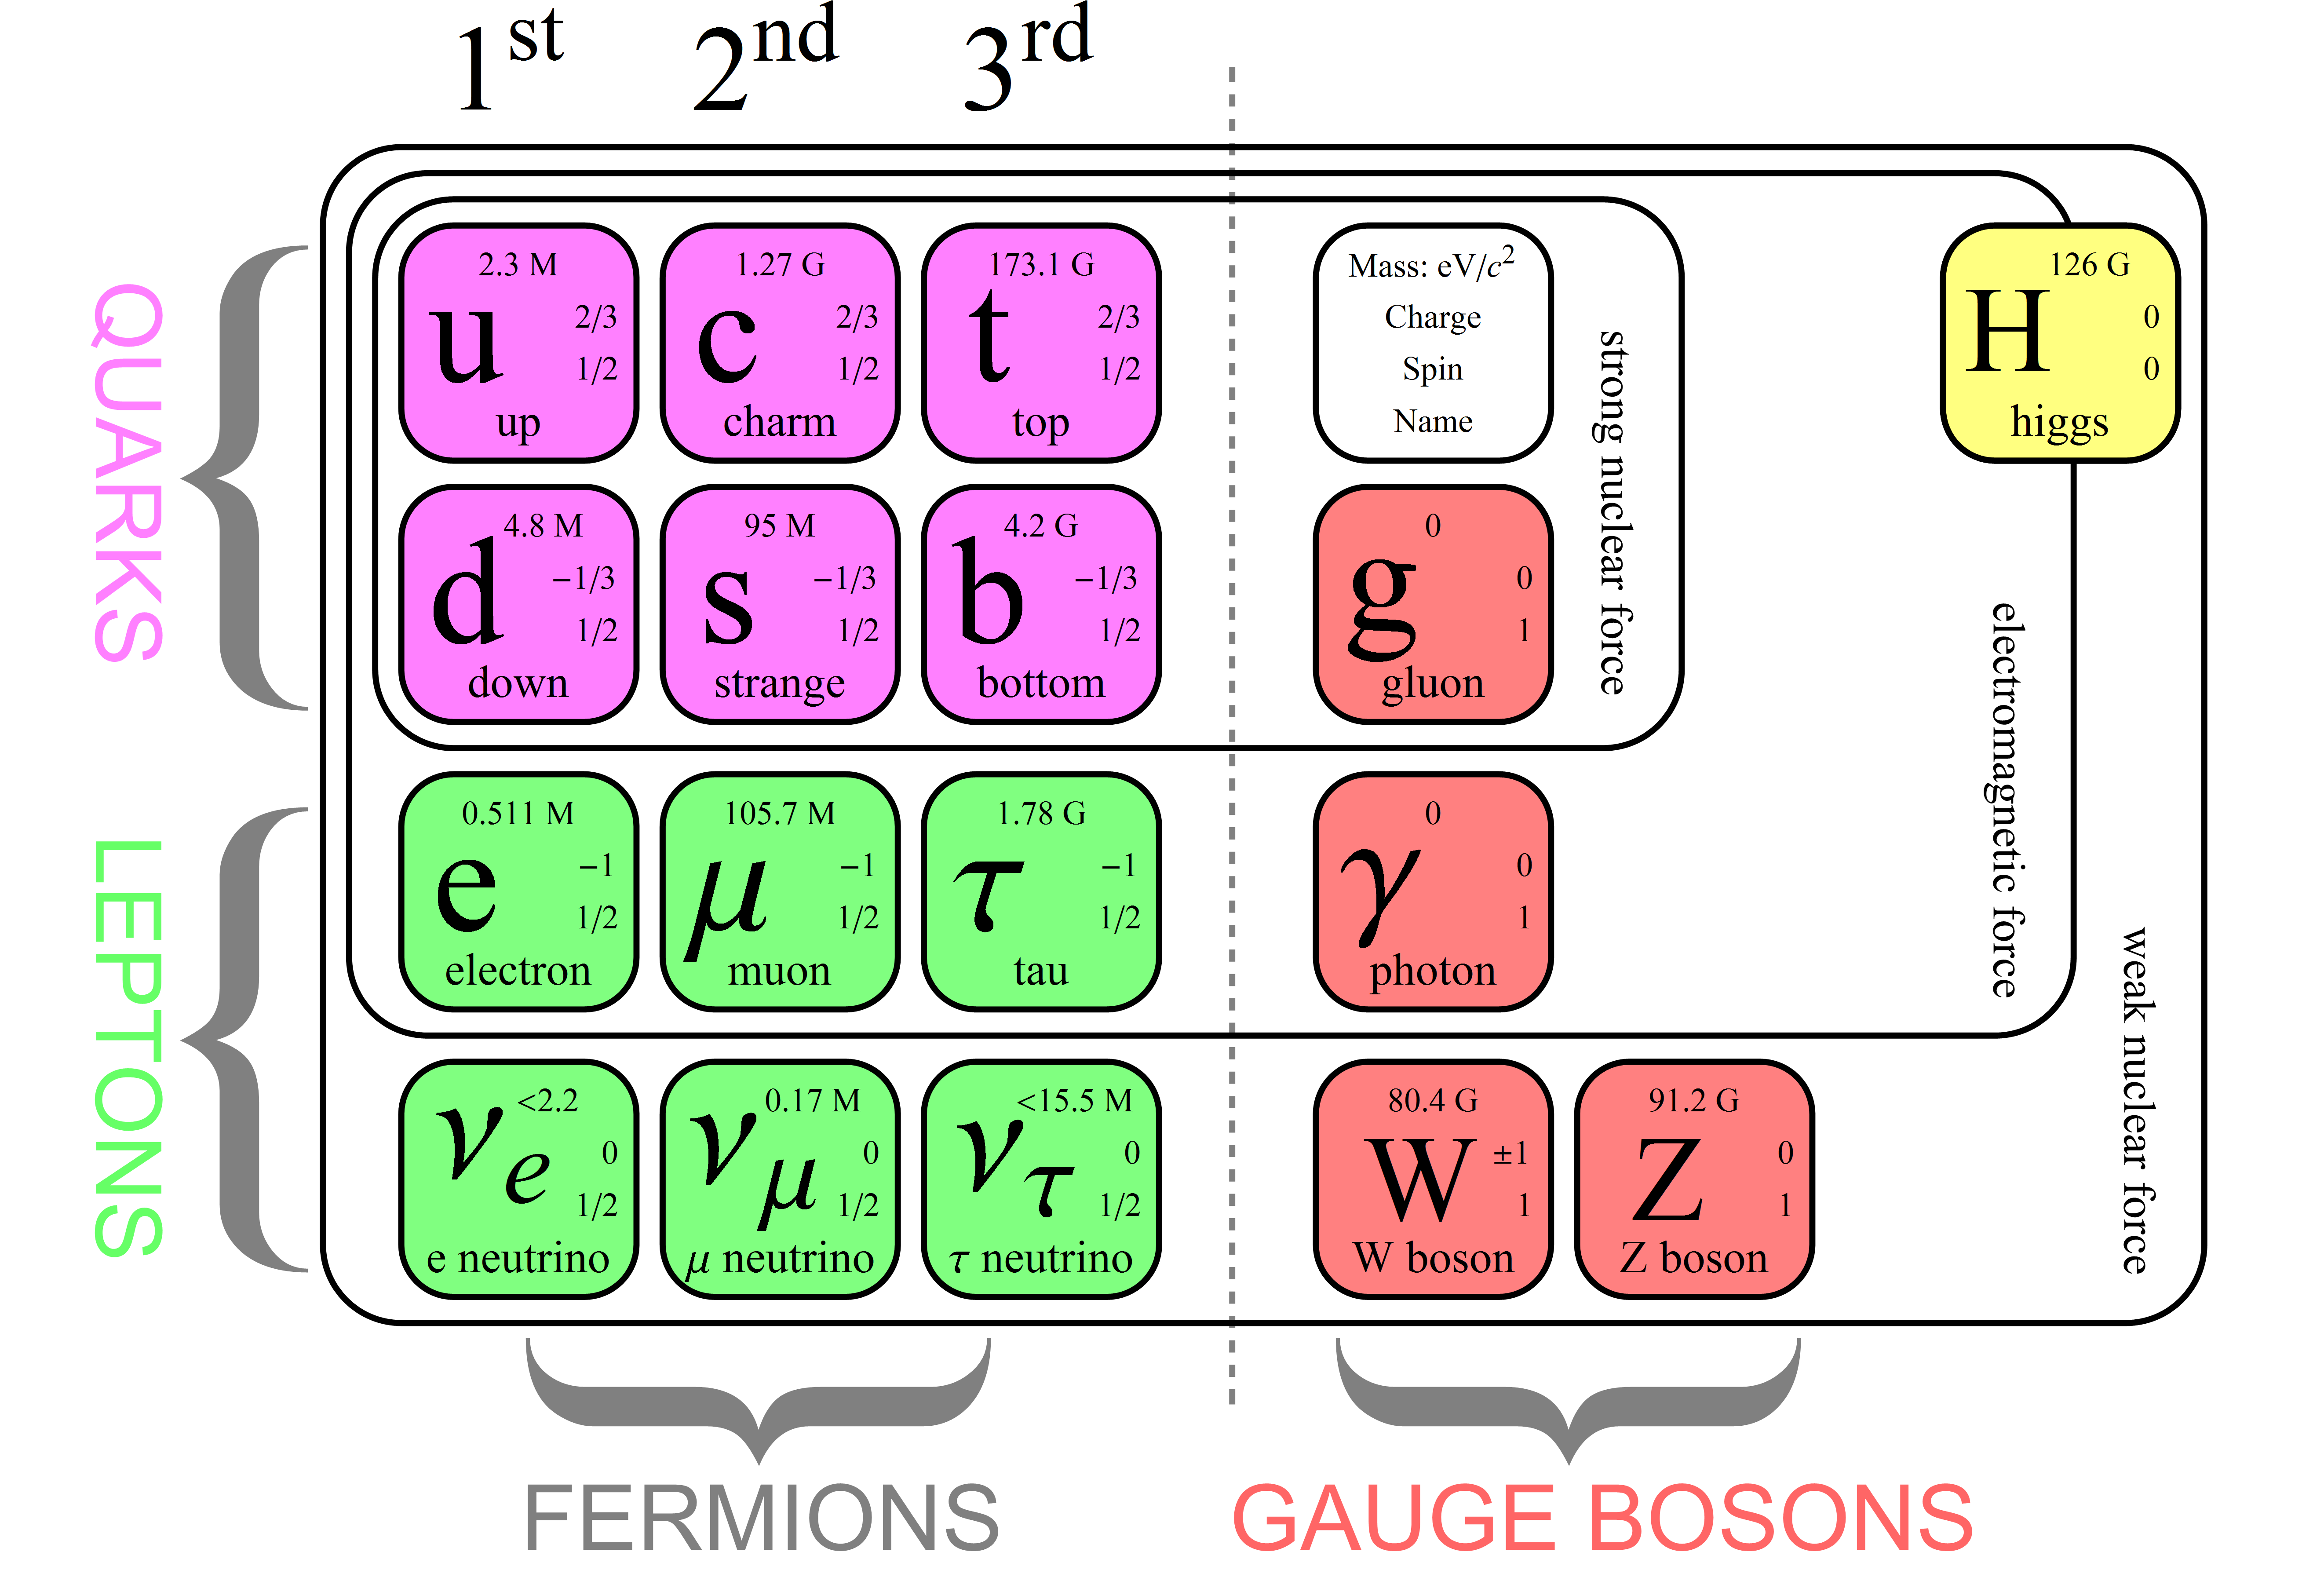
\includegraphics[width=0.98\textwidth]{./plots/SM.png}
  \caption{The particles of the Standard Model.}
  \label{fig:SMParticles}
\end{figure}

\ \\There are 12 fermions representing the constituents of matter. They have a semi-integer spin ($1/2$) and they can be divided into two categories: quarks and leptons. The quarks have fractional electric charges and form barions and mesons. They six quarks are up ($u\,^{+2/3}$), down ($d\,^{-1/3}$), charm ($c\,^{+2/3}$), strange ($s\,^{-1/3}$), top ($t\,^{+2/3}$), and bottom ($b\,^{-1/3}$). The three electrically-charged leptons have a negative charge: the electron ($e\,^{-}$), the muon ($\mu\,^{-}$), and the tau lepton ($\tau\,^{-}$). These have corresponding neutrally-charged leptons caled neutrinos ($\nu_e\,^0$, $\nu_\mu\,^0$, $\nu_\tau\,^0$). These particles form matter. For each matter particle there is an anti-matter particle that has an opposite electric charge. 

\ \\Fermions interact with each other via the echange of other elementary particles called bosons. Bosons are carriers of the elementary forces and have an integer spin ($1$). There are eight type of gluons ($g$) that carry the strong force. The photon ($\gamma$) is responsible for the electromagnetic force. The \Wplus, \Wminus~and the \Zzero~bosons carry the weak force. 

\ \\There is also another type of boson, a scalar elementary particle of spin zero (0), called the Higgs boson. The Higgs boson is the latest elementary particle discovered, in 2012, by the ATLAS and CMS detectors at CERN. It is predicted by the mechanism that explains how the elementary particles acquire mass.

\subsection{The top quark}
\label{sec:TopQuark}

The top quark ($t$) is a very interesting elementary particle to study, for several reasons. It is the heaviest particle from the SM, with a mass \mt=173.3~\GeVcc. This implies the top quark has the highest Yukawa coupling constant. The top quark decays very quickly ($\tau=10^{-25}$ s), before having the time to hadronize, meaning to form stable hadrons. Therefore it is the only quark that can be studied alone. It is observed indirectly through its decay products. The top quark was discovered in 1994 independently by the CDF and DZero experiments at FermiLab in proton-antiproton ($p\bar{p}$) collisions at $\sqrt{s}=1.8$ TeV.

\ \\Measuring the top-quark properties is key to test the validity of the SM. The ATLAS and CMS experiments at CERN measure the properties of the top quark in great detail. If deviations are found in the top quark properties with respect to the SM predictions (\emph{e.g.} different cross-sections), it implies the existence of new physics phenomena beyond the Standard Model (BSM). This would produce a revolution in particle physics, as the SM has not been contradicted by any experiment since its creation in the 1960s. 

\ \\The top quarks are produced in pairs by strong interactions. The Feynman diagrams for the leading order are illustrated in Figure~\ref{fig:TopQuarkFeynmanDiagrams}. At the LHC the quark-antiquark annihilation (left) represents 10\% of the cases, while the gluon-gluon fusion (center and right) represent 90\% of cases. The LHC has a very high luminosity and produces large quantities of top quarks. For this reason the LHC is considered to be also a top-quark factory.

\begin{figure}[h]
  \centering
  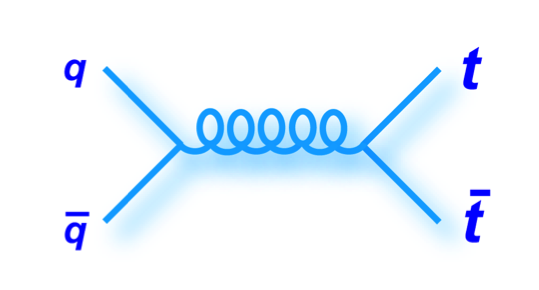
\includegraphics[width=0.32\textwidth]{../presentation/plots/ttbar_1.png}
  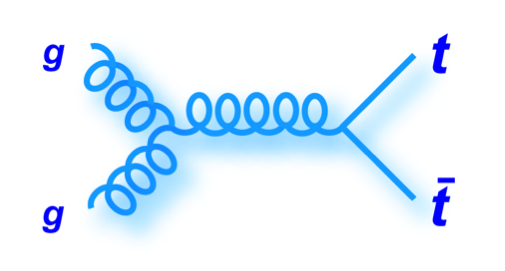
\includegraphics[width=0.32\textwidth]{../presentation/plots/ttbar_2.png}
  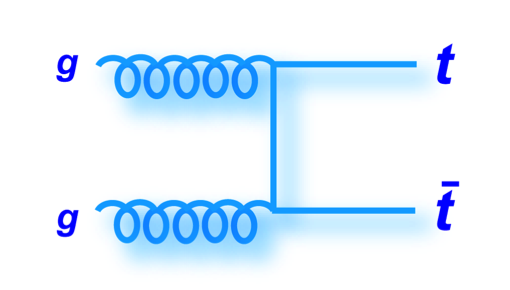
\includegraphics[width=0.32\textwidth]{../presentation/plots/ttbar_3.png}
  \caption{The Feynaman diagrams for the top-quark pair production. At the LHC the quark-antiquark annihilation (left) represents 10\% of the cases, while the gluon-gluon fusion (center and right) represent 90\% of cases.}
  \label{fig:TopQuarkFeynmanDiagrams}
\end{figure}

\ \\The top quark decays in almost 100\% of the time in a \Wboson~and a bottom ($b$) quark. The $W$ boson can decay either to a pair of a quark or an antiquark ($W\rightarrow q\bar{q}$), or to a pair of leptons ($W \rightarrow e\bar{\nu}_e$, $W \rightarrow \mu\bar{\nu}_\mu$, $W \rightarrow \tau\bar{\nu}_\tau$). The $\tau$ lepton decays further leaving as a visible signature in the detector an electron, a muon or two quarks. Since there are two top quarks, they decay to two \Wboson~bosons and two $b$ quarks. Quarks hadronise and appear in the detector as streams of collimated particles called jets. 

\ \\Counting the number of charged leptons (electrons or muons), the top quark events can be grouped into three categories: di-lepton, lepton+jets (one lepton plus jets), and all-hadronic (only jets). The percentage of decay for each case, called branching ratio (BR) is presented in the left-hand side of Figure~\ref{fig:TopQuarkDecay}. In this report we study the subset of the di-lepton with an electron or a muon. The \ttbaremu~decay is present in only 2\% of the cases. It is advantageous because the background is very low comparing to others decay channels. The background comes in most of the cases from the \Zboson~boson decay plus other jets. The full Feynman diagram of production and decay of the \ttbaremu~is presented in the right-hand side of Figure~\ref{fig:TopQuarkDecay}. The latest ATLAS paper on the \ttbaremu~analysis is presented in~\cite{ttbaremu}.

\begin{figure}[h]
  \centering
  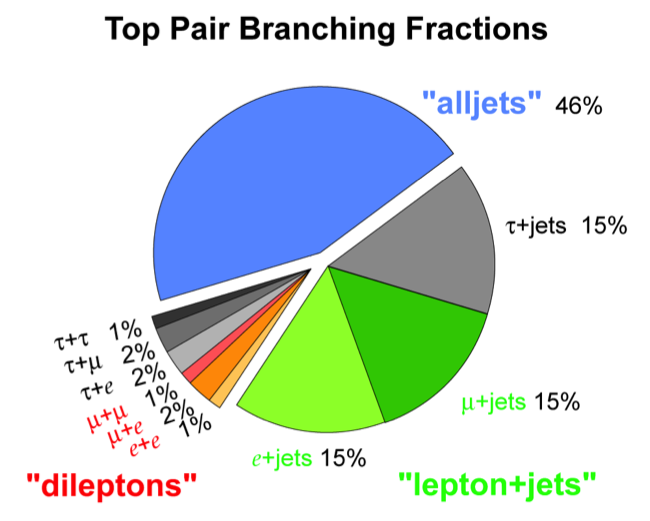
\includegraphics[width=0.47\textwidth]{../presentation/plots/ttbar_5.png}
  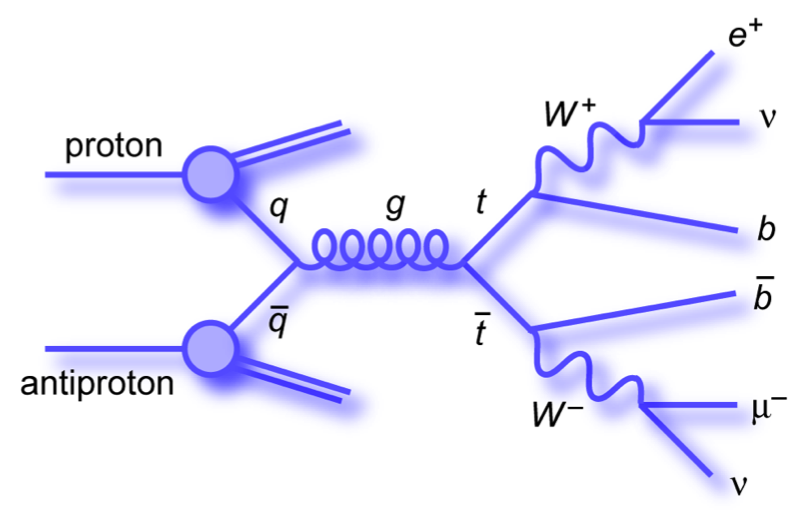
\includegraphics[width=0.47\textwidth]{../presentation/plots/ttbar_4.png}
  \caption{Left: the pie chart of the top-quark pair decay. Right: the Feynman diagram including production and decay of the \ttbaremu~process.}
  \label{fig:TopQuarkDecay}
\end{figure}

\subsection{The experimental setup}
\label{sec:ExperimentalSetup}

The experimental setup used in this study is from the ATLAS experiment at CERN.

\ \\At the moment, the Large Hadron Collider (LHC), which is situated at CERN, is the most powerful proton-proton collider in the world, as illustrated in Figure~\ref{fig:LHC}. After the Tevatron and the Large Electron-Positron Collider (LEP) era, a new machine was needed for new discoveries in particle physics. The LHC was designed to achieve a center-of-mass energy $\sqrt{s}=14\,TeV$. Two of the biggest goals of the LHC are to study the Standard Model and to test its validity.  

\begin{figure}[h]
  \centering
  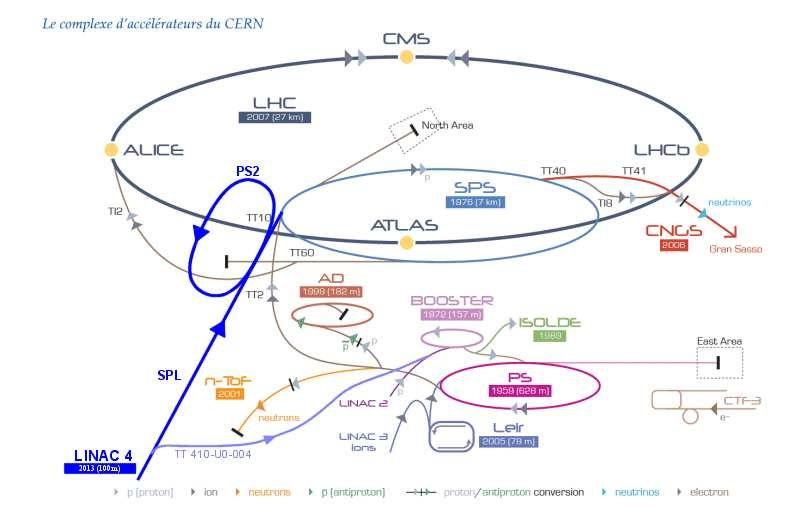
\includegraphics[width=0.5\textwidth]{plots/LHC.png} 
  \caption{The LHC Accelerator Complex System.}
  \label{fig:LHC}
\end{figure}

\ \\This project is affiliated to the international collaboration of the A Toroidal LHC ApparatuS (ATLAS)~\cite{ATLAS}. ATLAS is the largest of the four LHC detectors. ATLAS is one of the two general-purpose particle physics detectors at the LHC, the other being CMS. The two detectors and collaborations perform a similar research program. A new discovery must be observed by both detectors to be believed as true. ATLAS and its subdetectors is illustrated in Figure~\ref{fig:ATLAS}.

\begin{figure}[h]
  \centering
  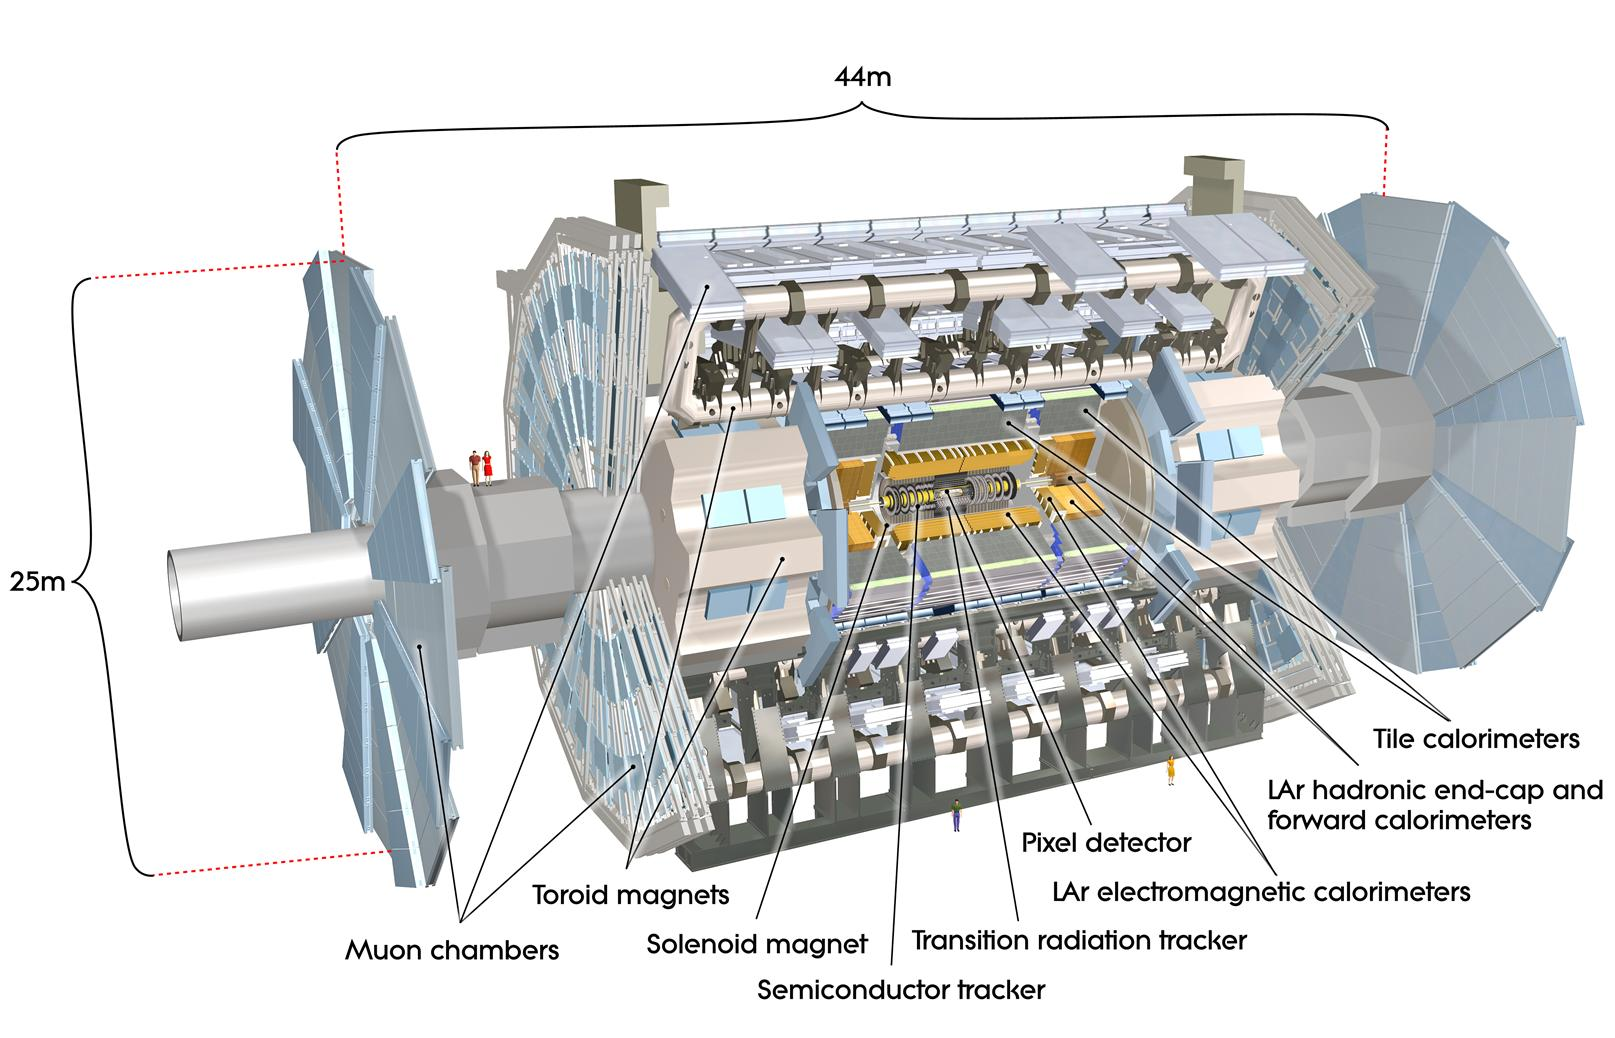
\includegraphics[width=0.5\textwidth]{plots/ATLAS.jpg} 
  \caption{The ATLAS detector and its sub-detectors.}
  \label{fig:ATLAS}
\end{figure}

\ \\ This report presents results obtained using 43076 simulated events of the \ttbaremu~process within the ATLAS experiment~\cite{RootFile}. After an event selection, for each event there is the information available at the reconstructed stage (measured) stage and at the truth (generated) stage. The study focuses on the jet with the highest transverse momentum (\pt), also called the leading jet, in the interval from 0 to 500 \GeV, with a constant bin width of 20 \GeV, which results in 25 bins in total.

\section{Unfolding methods}
\label{sec:UnfoldingMethods}

As introduced in Section~\ref{sec:Introduction}, after the discovery of the Higgs boson at CERN, it becomes even more important to test the validity of the SM via precision measurements on SM particles. Properties of such particles are measured in the ATLAS detector. The measured quantities are close, but not identical to the true value of the quantities these particles had in reality in nature, due to detector smearing effects. Every measurement has a total uncertainty, formed from statistical and systematic uncertainties. It is therefore important to have a mechanism to reverse the detector smearing by inferring the true value of a quantitity given the measured value of the quantity. Such mechanism is called \emph{unfolding} and is the topic of this project. The estimated true quantity from unfolding the reconstructed quantity is then compared with the theoretical prediction. If a difference is observed even after taking into account the experimental and theoretical uncertainties, a deviation from the SM would be observed. If confirmed at five standard deviations ($\sigma$), it would represent a revolution in particle physics. Therefore, unfolding methods are key to testing the SM and searching for new physics beyond the Standard Model (BSM). An introduction to unfolding methods for particle physics can be studied in~\cite{UnfoldingStatSchool}.

\ \\There are two types of unfolding methods: a traditional method using a binned 2D hisogram representing a migration matrix for one variable, and machine learning predicting a continuous function for several variables, as illustrated in Figure~\ref{fig:TwoUnfoldingTechniques}. 

\begin{figure}[t]
  \centering
  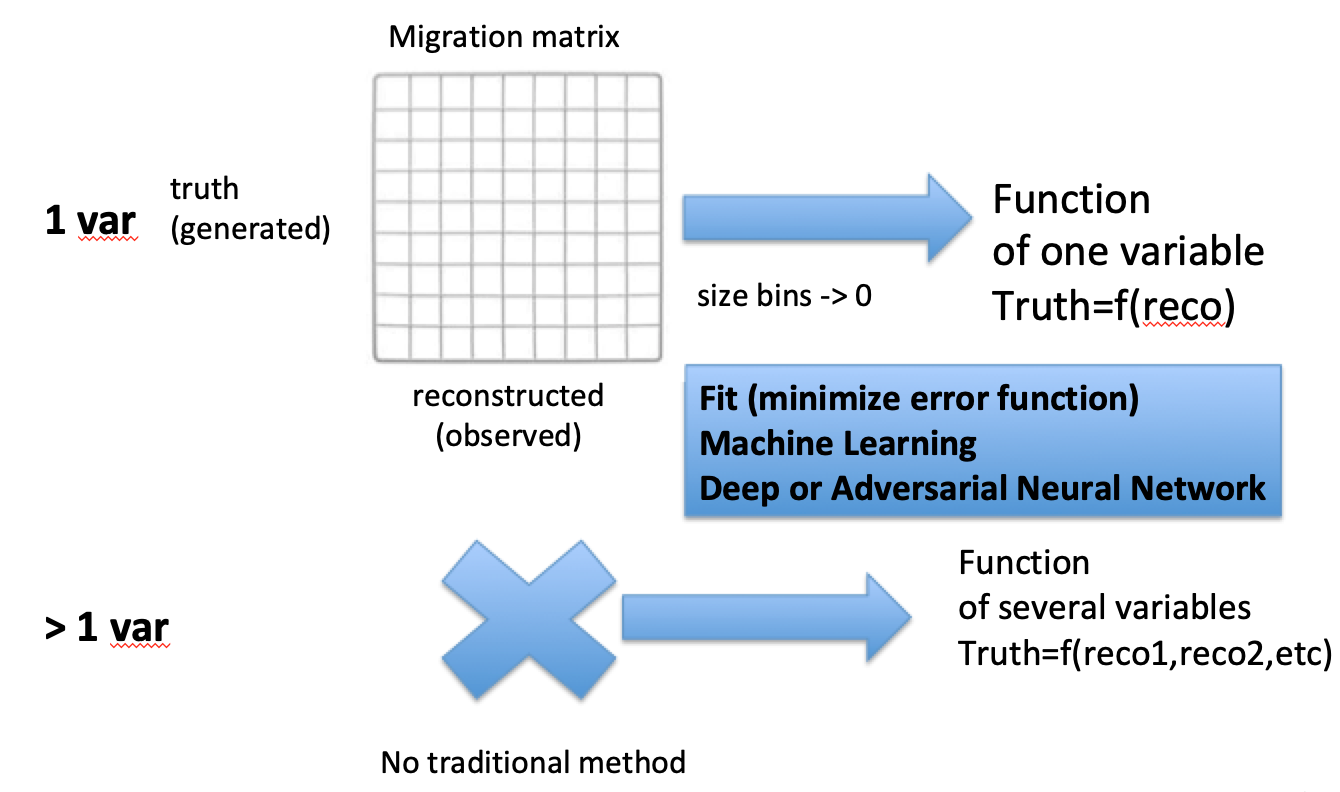
\includegraphics[width=0.98\textwidth]{../presentation/plots/Unfolding_Traditional_ML.png}
  \caption{Comparison of the two unfolding method: traditional (migration matrix, one variable) and machine learning (continuous function, several variables).}
  \label{fig:TwoUnfoldingTechniques}
\end{figure}

\subsection{The traditional method: the migration matrix}
\label{sec:UnfoldingMigrationMatrix}

In the traditional method, only one quantity is used at a time. In simulated data, there are two versions for each quantity of the same event: a reconstructed quantity (or reco, which for measured data would be the observed quantity) and the generated quantity (that would be the truth, or the true value in nature). An interval and binning is chosen for this variable. A 2D histogram is filled, as a given event is in a particular bin in the reco on the horizontal and in a particular bin in the truth on the vertical. The histogram is called a migration matrix, as it describes how a quantity migrates from a particular bin in the reconstructed to another bin (usually nearby) for the truth. Ideally, this matrix is diagonal. In practice, there are non diagonal values that are non zero. Such a matrix is used in the traditional unfolding. 

\ \\For the simulated dataset studied in this report, the migration matrix of the leading jet \pt~bin value is presented in Figure~\ref{fig:MigrationMatrix}, taken from~\cite{ReportYichenLi}. There are 25 bins possible for the leading jet \pt~values between 0 and 500 \GeV, with 20 \GeV~bins. The number in a cell represents the probability (as a percent) of an event in the truth bin \emph{i} to be reconstructed in a reco bin \emph{j}. The numbers are normalised so that the sum of values on a horizonthal row is 100 (percent). The more diagonalizable matrix, the easier unfolding will be. Events are migrating from one truth bin to other bins for reco, and vice-versa.

\begin{figure}[h]
  \centering
  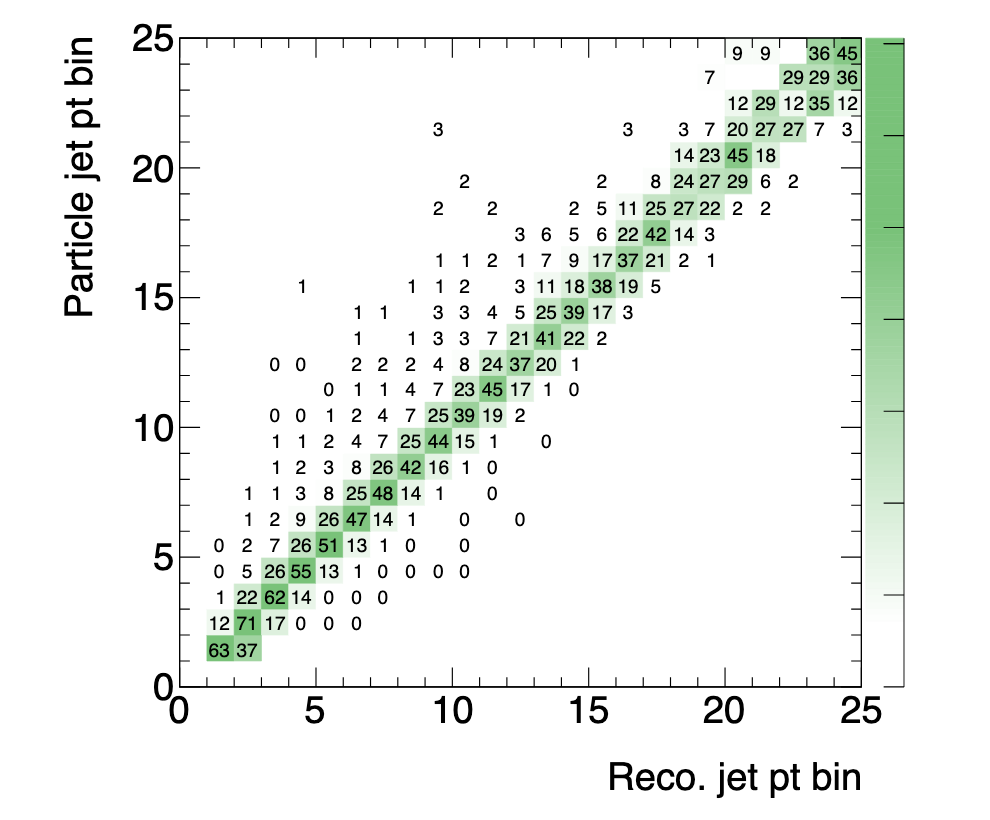
\includegraphics[width=0.8\textwidth]{../presentation/plots/jetPt_migration_matrix.png}
  \caption{The leading particle jet \pt~bin versus the leading reco jet \pt~bin, for the same events of this study~\cite{ReportYichenLi}.}
  \label{fig:MigrationMatrix}
\end{figure}

\ \\Traditional unfolding is an iterative Bayesian process. After four iterations, the unfolded results are presented in Figure~\ref{fig:2DMigrationMatrix}, taken from~\cite{ReportYichenLi}. The left hand-side presents the jet distribution for truth and for the truth unfolded from the reco, while the right-hand side presents the coefficients matrix in a 2D histogram format.

\begin{figure}[h]
  \centering
  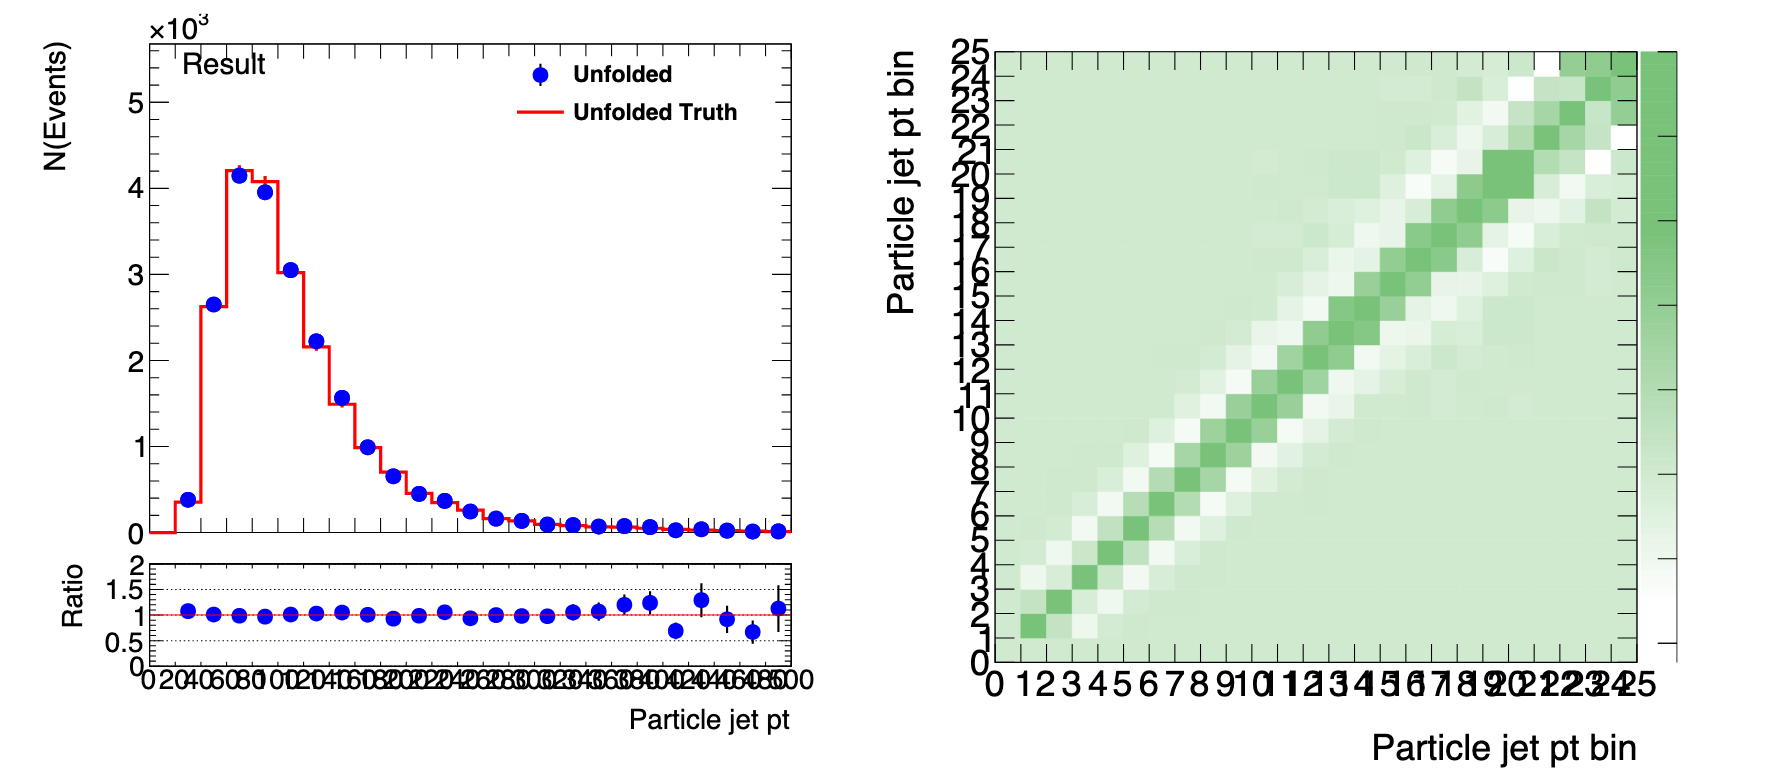
\includegraphics[width=0.98\textwidth]{./plots/TraditionalUnfoldingResults.png}
  \caption{Traditional unfolding results for the leading jet \pt~in a 1D and 2D histogram.}
  \label{fig:2DMigrationMatrix}
\end{figure}

\subsection{The new method: machine learning}
\label{sec:UnfoldingMachine Learning}

As the bin width is decreased continuously closed to infinitesimal values, the migration matrix becomes a function of one variable that maps each reco quantity to its truth quantity. This is equivalent to a function \texttt{truth=f(reco)}. But it still can have only one variable. Finding such a function is in general found via minimizing an error function over some parameter space, a process which is also called a \emph{fit}. A fit with even several variables can be done successfully via machine learning, where a functions is learned of the form \texttt{truth=f(reco1, reco2, etc.)}. 

\ \\A new approach of unfolding via machine learning has been proposed by A. Glazov at DESY Hamburg~\cite{AGlazov}, together with a code example~\cite{AGlazovCode} of training a (deep) neural network on toy simulated data using TensorFlow~\cite{TensorFlow} via ~\cite{Keras} in \texttt{Python}, using numpy~\cite{numpy}, as illustrated in Figure~\ref{fig:CodeSoftware}. 

\begin{figure}[h]
  \centering
  
\includegraphics[width=0.30\textwidth]{../presentation/plots/TensorFlow_Keras.png}
  
\includegraphics[width=0.30\textwidth]{../presentation/plots/Python.png}
  \caption{A modern (deep) neural network is typically trained in Keras with a TensorFlow backend, run in Python, using numpy.}
  \label{fig:CodeSoftware}
\end{figure}

\ \\The goal of the study is to adapt this example to use real data coming from the jet \pt~distribution from the \ttbaremu~analysis. We use this \texttt{.root} flat tree~\cite{RootFile}. This file contains both the reconstructed and truth jets, already matched. Meaning the i$^{\rm th}$ event from reco, corresponds to the i$^{\rm th}$ event from truth. Each jet collection contains jets already the jets ranked by \pt. We take index 0 to consider the leading reco jet and the leading truth jet.

\ \\Using this approach, the leading jet \pt~unfolding is formulated in the example illustrated in Figure~\ref{fig:PhysicsProblem}. For both reco and truth, \pt~larger than 500 \GeV~are changed to 499.999 \GeV, and thus moved to the last bin. This is equivalent to moving the overflow bin of a histogram to the last bin of a histogram. The truth and reco are thus ensured to have the same number of potential bins (25), given the 0-500 \GeV~range and the bin width of 20 \GeV. The simplest case of only one variable is considered: the jet \pt, or more exactly, the jet \pt~bin. Let's consider an example for the reconstructed jet (the input of unfolding) and the truth jet (the output of unfolding).

\begin{figure}[h]
  \centering
  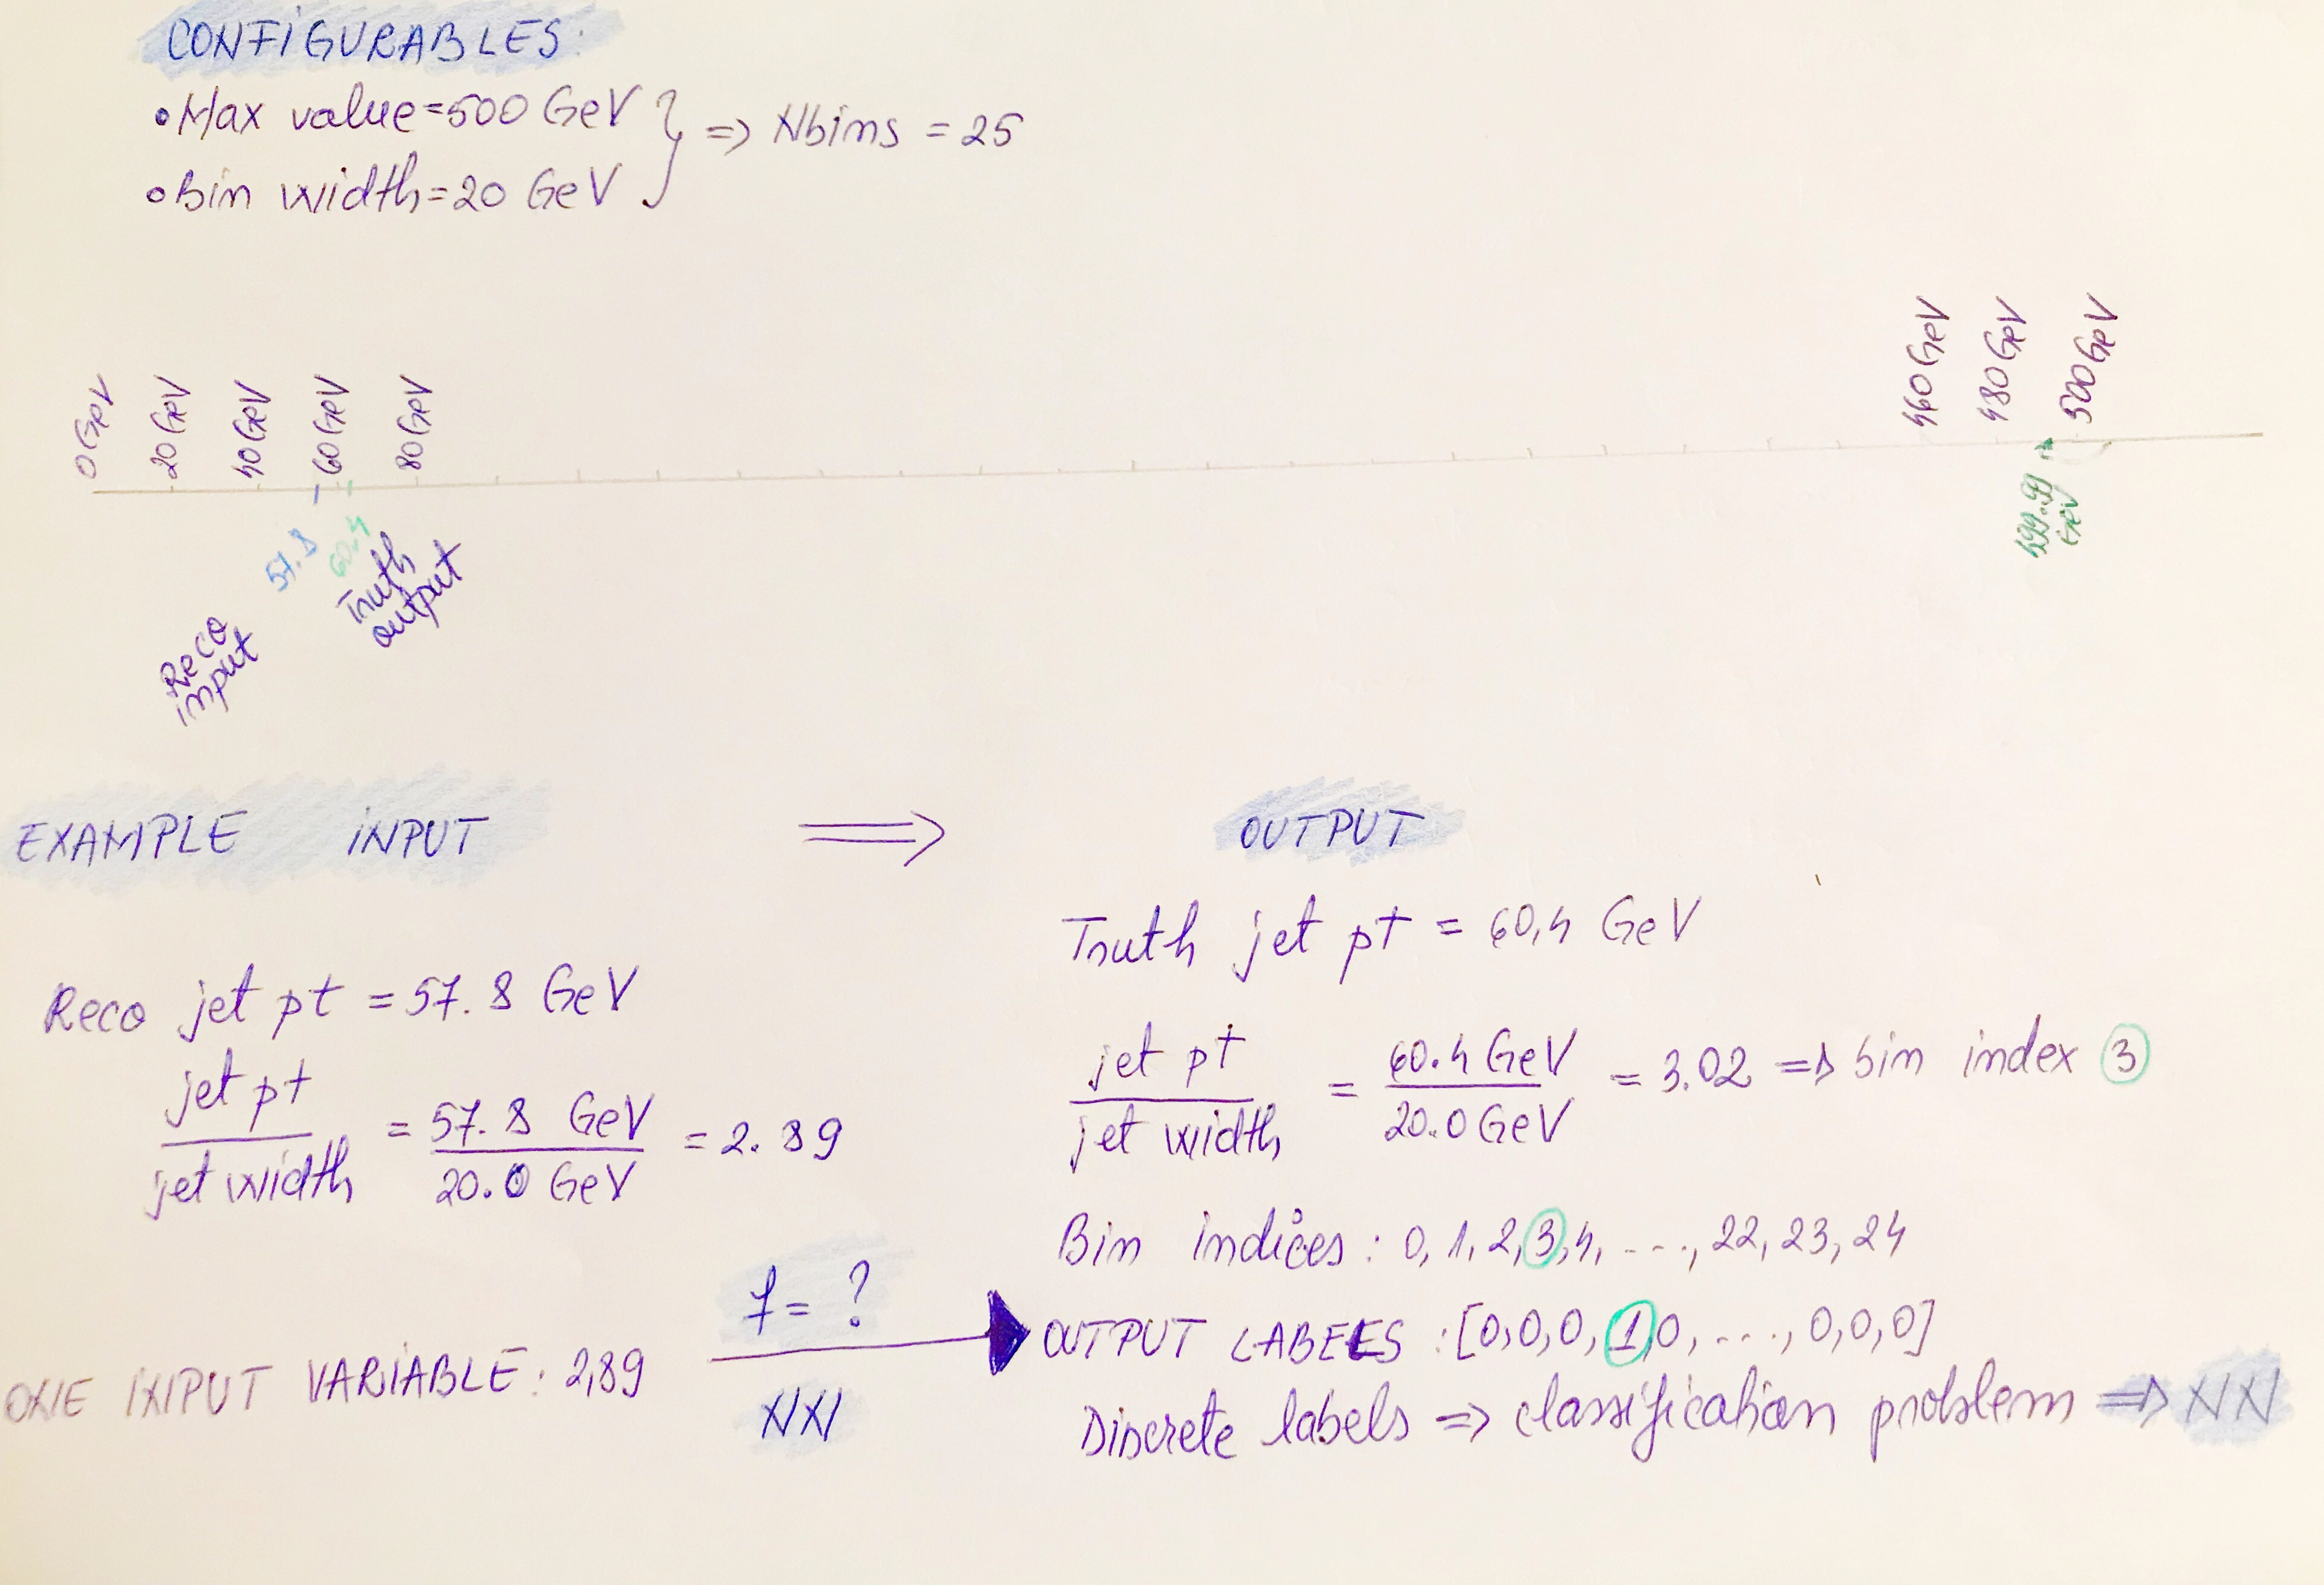
\includegraphics[width=0.98\textwidth]{../presentation/plots/PhysicsProblem.jpg}
  \caption{Exemple of problem posing for the leading jet \pt~unfolding with the machine learning approach of~\cite{AGlazov}~\cite{AGlazovCode}.}
  \label{fig:PhysicsProblem}
\end{figure}

\ \\For a reconstructed jet, the ratio between the \pt and the bin width represents the input to the machine learning. For example, for a 57.8 \GeV~jet, the value is 2.89. The jet would fit in the third bin, or the bin of index 2 (index values start at 0).

\ \\For a truth jet, things are similar, but a bit more complex. Imagine the same jet has a different value for the truth, equal with 60.4 \GeV. Dividing by the bin width, 3.02 is obtained. The truth jet falls in the fourth bin, or the bin of index 3. The goal of the unfolding via machine learning is to learn and then predict, or infer, this number 3. 3 is only one possible answer out of finate number of posibilities corresponding to the 25 bins. Each bin can be considered one category of potential output. Each jet belongs to only one category. This problem is called classification and can indeed be solved via machine learning. To note that in this method is not attempted to predict exactly the \pt~of the truth jet. There would be a continous interval of possible values. Such a problem is called regression. It is also possible to be solved via machine learning, but it is more complex. 

\ \\In this project we choose to predict only the bin where the jet \pt~falls into, or a multi-label classification or categorization problem. The categorisation is a common problem solved via modern Machine Learning methods. Possible methods could be Boosted Decision Trees (BDT)~\cite{JoshuaBendavid}~\cite{AndrewNg} and Artificial Neural Networks (ANN or NN)~\cite{AndrewNg}. 

\ \\Classification is usually binary, distinguishing between two possibilties: signal or background, good or bad, 1 or 0. It is therefore technically easier to formulate that for the input of 2.89, the output not as the bin index 3, but as a range of 25 values, each being 0 or 1, all of them being zero, except for the index 3, where the value is 1, as illustrated in Table~\ref{tab:InputOutput}. Finding such a function connecting this type of input to this type of output for all the jets in the event is done via a deep neural network (NN) training in this project. The NN will try to learn and predict for each of the 25 positions the values of 0 or 1. But in practice it will output for each position a real number with a value between 0.0 and 1.0. The NN will return the probability that for a given jet its \pt~falls in any of these bins. The total probability for all bins must be 1.

\begin{table}[h!]
  \centering
    \begin{tabular}{|l|l|l|}
      \hline
      \textbf{Jet} & \textbf{Input} & \textbf{Output}\\
      \hline
      Physics & 2.89 & 3.02 \\
      Classification & 2.89 & 3 \\
      Neural Network & 2.89 & [0,0,0,1,0,0,...,0,0,0] \\
      \hline
    \end{tabular}
 \caption {Example of jet reco (input) and truth (output) from physics to the NN.}
\label{tab:InputOutput}
\end{table}

\ \\The input and output layers of the NN are fixed by the problem formulation. The architecture of the middle layers can be optimised for the specific problem. The NN architecture suggested in the code example~\cite{AGlazovCode} is denoted in this report the old NN. Several architectures and NN hyper-parameters have been optimised in this study by changing one parameter while keeping all the rest constant. The best of the many NNs tried is denoted in this report the new NN. 

\ \\The following section~\ref{sec:NeuralNetworks} will describe the optimisation process and compare the two NNs in terms of the NN-specific figures of merits of accuracy and loss. After that, the section~\ref{sec:Results} will compare the two NNs in terms of the unfolding of the leading jet \pt.

\section{Neural Networks}
\label{sec:NeuralNetworks}

\subsection{The method}
\label{sec:Method}

My first step was to study a code example using some toy data in a JupyterNotebook~\cite{AGlazov}. At the beginning I ran the code on a cloud (Swan). 

\ \\The next step was to run it on \texttt{lxplus}. For this it was needed to run after \texttt{ssh}-ing to a \texttt{lxplus} machine a singularity command~\cite{Singularity} and then to my own laptop.

\ \\To train the neural network it was needed to use the Python library Keras~\cite{keras} and for backend TensorFlow~\cite{tensorflow}. My method of sampling was implemented using numpy~\cite{numpy}.

The goal of this project is to adapt a code example of machine learning unfolding (MLUnfolding) using toy data to use it for the jet energy reconstruction of \ttbaremu~analysis.

\ \\In this project one of the problems that we want to solve is the correction of detector smearing using Machine Learning (ML). I have implemented this method using a sequential Neural Network. The unfolding corresponds to an inversion of the migration matrix. Unfolding is the procedure to infer the truth data (what happens in reality in nature) from the reconstructed data (observed and measured in our experiment by our detector). The categorisation is a common problem for the modern Machine Learning methods. Possible methods could be Boosted Decision Trees (BDT) and Artificial Neural Networks (ANN), or in short Neural Networks (NN). NNs with various architectures can be tried for the unfolding problem. The unfolding involves several iterative steps of ML using a NN training in TensorFlow via Keras, in Python. The NN takes as input the reconstructed values, and has as output the truth values.

\ \\The goal of the study is to adapt this example to use real data coming from the jet \pt~distribution from the \ttbaremu~analysis. We use this \texttt{.root} flat tree~\cite{RootFile}. This file contains both the reconstructed and truth jets, already matched. Meaning the i$^{\rm th}$ event from reco, corresponds to the i$^{\rm th}$ event from truth. Each jet collection contains jets already the jets ranked by \pt. We take index 0 to consider the leading reco jet and the leading truth jet.

\ \\Given the leading jet \pt~as a continuous reco value, we want to find out in which jet \pt~bin does the truth jet falls. The jet bin is configurable, say 10 \GeV, or 20 \GeV. The input is a continuous value, but the output is a discrete value, that can take values from 0 to 24 if we consider 20 \GeV~bins from 0 to 500 \GeV. For example, bin index 0 contains jets with \pt~from 0 to 20 \GeV, bin index 1 contains jets with \pt~from 20 \GeV~to 40 \GeV, \emph{etc.}. Jets with \pt~larger than 500 \GeV~have values set by hand to 499.999 \GeV, and enter in the last possible bin index, number 24. It is equivalent to moving the overflow bin of a histogram to the last bin of the histogram. 

\ \\Given the output can take any value from 0 to 24, the problem we try to solve is a classification, and the possible labels are not only two (as in a simple signal to background classification, typically used in ATLAS), but a more complex one, with 25 labels. The NN will return the probability that for a given jet its \pt~falls in any of these bins. The total probability for all bins must be 1.0. This is ensured by the \emph{softmax} activation function for the last layer of the NN. We then consider the bin with the largest probability as our choice by the NN. The predicted bin value can then be compared with the true bin value when making the plots of this project.

\ \\To optimize the NN performance, we take as input in fact not the jet \pt, but the jet \pt~divided by the bin width. This is the jet \pt~bin as a real value. Making things more consistent with the output being the integer jet \pt~bin value for the truth.

\ \\ Neural Networks are an example of Machine Learning. In this way the computers learn a solution for a problem without being explicitly programmed. The two main classes of ML are supervised and unsupervised. 
In this project I used supervised ML. ......~\cite{AndrewNg}.

\ \\If we have the function Pi(y), a multidimensional highly non-linear, an efficient way to do this procedure is with an NN. This was inspired by the brain structure, which contains millions of neurone cells forming a network with electrochemical impulses passing between them. An artificial neural network formed by a number of interconnected artificial \emph{neurons}, or "nodes" respects this architecture. 

\ \\A network is formed by several ayers of nodes connected in series. Each node takes a weighted linear combination of the outputs from nodes of the previous layer, applies "activation function", then outputs the result do the next layer~\cite{AndrewNg}.

\ \\Using a "loss" function we can describe the difference between the predicted and real outputs, like the mean squared error between real and predicted. The weights associated with each node is modifies via an algorithm, and from here we can deduce that the loss function decreases and training increases.

\ \\We know from The \emph{Universal Approximation Theorem} that a neural network with one \emph{hidden layer} of nodes between input and output can in principle approximate any N-dimensional function to an arbitrary degree of accuracy, given a sufficiently large (though finite) number of nodes. 

\ \\In practice it is more suitable to use multiple hidden layers connected in series~\cite{AndrewNg}.

\section{Results}
\label{sec:Results}

The shapes of the distributions of the truth and reco leading jet \pt~observables are very similar, but not identical (especially in the first bins), as illustrated in Figure~\ref{fig:jetPt} for the training set (left) and for the testing set (right).

\begin{figure}[h]
  \centering
  \includegraphics[width=0.49\textwidth]{../output_20GeV/NN_plot1D_train_jetPt_truth_reco.pdf}
  \includegraphics[width=0.49\textwidth]{../output_20GeV/NN_plot1D_test_jetPt_truth_reco.pdf}
  \caption{Overlay with ratio pad of the truth and reco leading jet \pt. Train and Test.}
  \label{fig:jetPt}
\end{figure}

Two figures of merit are used to optimise the NN hyper-parameters. The accuracy: the larger, the better (left: old NN; right: new NN). The loss (error) value: the smaller, the better (left: old NN; right: new NN). The overlaid train and test are very similar, which confirms the NNs are not overtrained.

\begin{figure}[h]
  \centering
  \includegraphics[width=0.49\textwidth]{../output_20GeV/NN_plot1D_optionTrainTest_accuracy_NN_l_A1_k_8_e_150_b_1000.pdf}
  \includegraphics[width=0.49\textwidth]{../output_20GeV/NN_plot1D_optionTrainTest_accuracy_NN_l_B3_k_4_e_150_b_200.pdf}
  \caption{Overlay with ratio pad of the truth and reco leading jet \pt. Old and new NN.}
  \label{fig:accuracyTrainTest}
\end{figure}

\begin{figure}[h]
  \centering
  \includegraphics[width=0.49\textwidth]{../output_20GeV/NN_plot1D_optionTrainTest_loss_NN_l_A1_k_8_e_150_b_1000.pdf}
  \includegraphics[width=0.49\textwidth]{../output_20GeV/NN_plot1D_optionTrainTest_loss_NN_l_B3_k_4_e_150_b_200.pdf}
  \caption{Overlay with ratio pad of the truth and reco leading jet \pt. Old and new NN.}
  \label{fig:lossTrainTest}
\end{figure}

Overlaying the two NN architectures, the old and new. The accuracy is the larger, the better.

\begin{figure}[h]
  \centering
  \includegraphics[width=0.49\textwidth]{../output_20GeV/NN_plot1D_train_accuracy_NN_final.pdf}
  \includegraphics[width=0.49\textwidth]{../output_20GeV/NN_plot1D_test_accuracy_NN_final.pdf}
  \caption{Overlay with old and new NN for the accuracy value (the smaller the better).}
  \label{fig:accuracyOldNew}
\end{figure}

\begin{figure}[h]
  \centering
  \includegraphics[width=0.49\textwidth]{../output_20GeV/NN_plot1D_train_loss_NN_final.pdf}
  \includegraphics[width=0.49\textwidth]{../output_20GeV/NN_plot1D_test_loss_NN_final.pdf}
  \caption{Overlay with old and new NN for the loss value (the larger the better). Train and test.}
  \label{fig:lossOldNew}
\end{figure}

The jet pt distribution as the index of the jet pt bin. True output (generated, truth) vs input (reconstructed). Used in traditional unfolding.

\begin{figure}[h]
  \centering
  \includegraphics[width=0.49\textwidth]{../output_20GeV/NN_plot1D_train_jetPtBin_NN_noTrained.pdf}
  \includegraphics[width=0.49\textwidth]{../output_20GeV/NN_plot1D_test_jetPtBin_NN_noTrained.pdf}
  \caption{Overlay ?. Train and test.}
  \label{fig:ptIndexNoTrained}
\end{figure}

The true output vs the predicted unfolded output by each NN architecture. The new NN architecture is closer to the true output than the old one.

\begin{figure}[h]
  \centering
  \includegraphics[width=0.49\textwidth]{../output_20GeV/NN_plot1D_train_jetPtBin_NN_final.pdf}
  \includegraphics[width=0.49\textwidth]{../output_20GeV/NN_plot1D_test_jetPtBin_NN_final.pdf}
  \caption{Overlay ?. Train and test.}
  \label{fig:ptIndexFinal}
\end{figure}

The predicted NN output minus the true output.  Both outputs are integers, representing bin indices. Therefore the difference is also an integer. The greater the count at zero difference, the better.  Top: train, bottom: test. Left to right, bin widths of 10, 20, 50, 100 GeV. The smaller the binWidth, the better is the new NN architecture relative to the old one.

\begin{figure}[h]
  \centering
  \includegraphics[width=0.49\textwidth]{../output_10GeV/NN_plot1D_train_outputPredictedMinusTrue_NN_final.pdf}
  \includegraphics[width=0.49\textwidth]{../output_10GeV/NN_plot1D_test_outputPredictedMinusTrue_NN_final.pdf}\\
  \includegraphics[width=0.49\textwidth]{../output_20GeV/NN_plot1D_train_outputPredictedMinusTrue_NN_final.pdf}
  \includegraphics[width=0.49\textwidth]{../output_20GeV/NN_plot1D_test_outputPredictedMinusTrue_NN_final.pdf}\\
  \includegraphics[width=0.49\textwidth]{../output_50GeV/NN_plot1D_train_outputPredictedMinusTrue_NN_final.pdf}
  \includegraphics[width=0.49\textwidth]{../output_50GeV/NN_plot1D_test_outputPredictedMinusTrue_NN_final.pdf}\\
  \includegraphics[width=0.49\textwidth]{../output_100GeV/NN_plot1D_train_outputPredictedMinusTrue_NN_final.pdf}
  \includegraphics[width=0.49\textwidth]{../output_100GeV/NN_plot1D_test_outputPredictedMinusTrue_NN_final.pdf}\\
  \caption{Overlay ?. Train and test.}
  \label{fig:binIndexPredictedMinusTruel}
\end{figure}

The 2D histogram migration matrix of the index of the jet pt. The closer to a diagonal matrix, the better.

\begin{figure}[h]
  \centering
  \includegraphics[width=0.49\textwidth]{../output_20GeV/NN_plot2D_train_outputTrue_input.pdf}
  \includegraphics[width=0.49\textwidth]{../output_20GeV/NN_plot2D_test_outputTrue_input.pdf}\\
  \includegraphics[width=0.49\textwidth]{../output_20GeV/NN_plot2D_train_outputTrue_outputPredicted_NN_l_A1_k_8_e_150_b_1000.pdf}
  \includegraphics[width=0.49\textwidth]{../output_20GeV/NN_plot2D_test_outputTrue_outputPredicted_NN_l_A1_k_8_e_150_b_1000.pdf}\\
  \includegraphics[width=0.49\textwidth]{../output_20GeV/NN_plot2D_train_outputTrue_outputPredicted_NN_l_B3_k_4_e_150_b_200.pdf}
  \includegraphics[width=0.49\textwidth]{../output_20GeV/NN_plot2D_test_outputTrue_outputPredicted_NN_l_B3_k_4_e_150_b_200.pdf}\\
  \caption{Overlay ?. Train and test.}
  \label{fig:2DMigrationMatrix}
\end{figure}

Traditional unfolding results. Plot taken from Fig. 5 of~\cite{ReportYichenLi}. Traditional unfolding: iterative bayesian unfolding with 4 iterations. 

\begin{figure}[h]
  \centering
  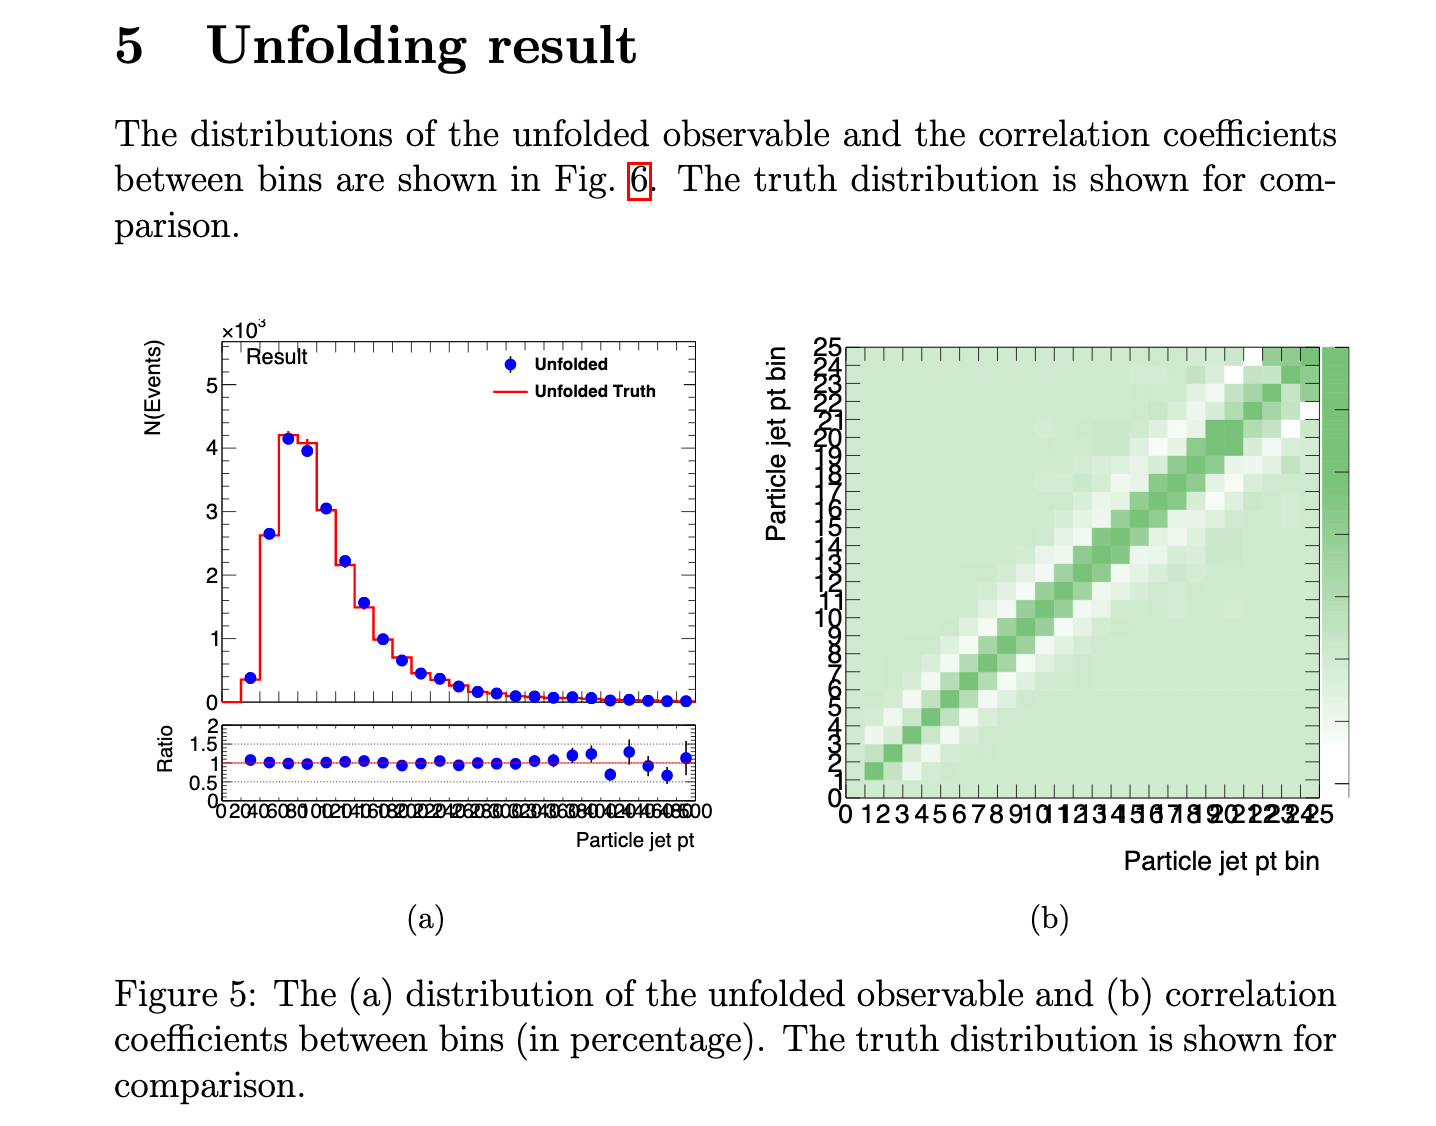
\includegraphics[width=0.49\textwidth]{../presentation/plots/TraditionalUnfolding.png}
  \caption{Traditional unfolding results.}
  \label{fig:2DMigrationMatrix}
\end{figure}

Defining the physics problem. 

\begin{figure}[h]
  \centering
  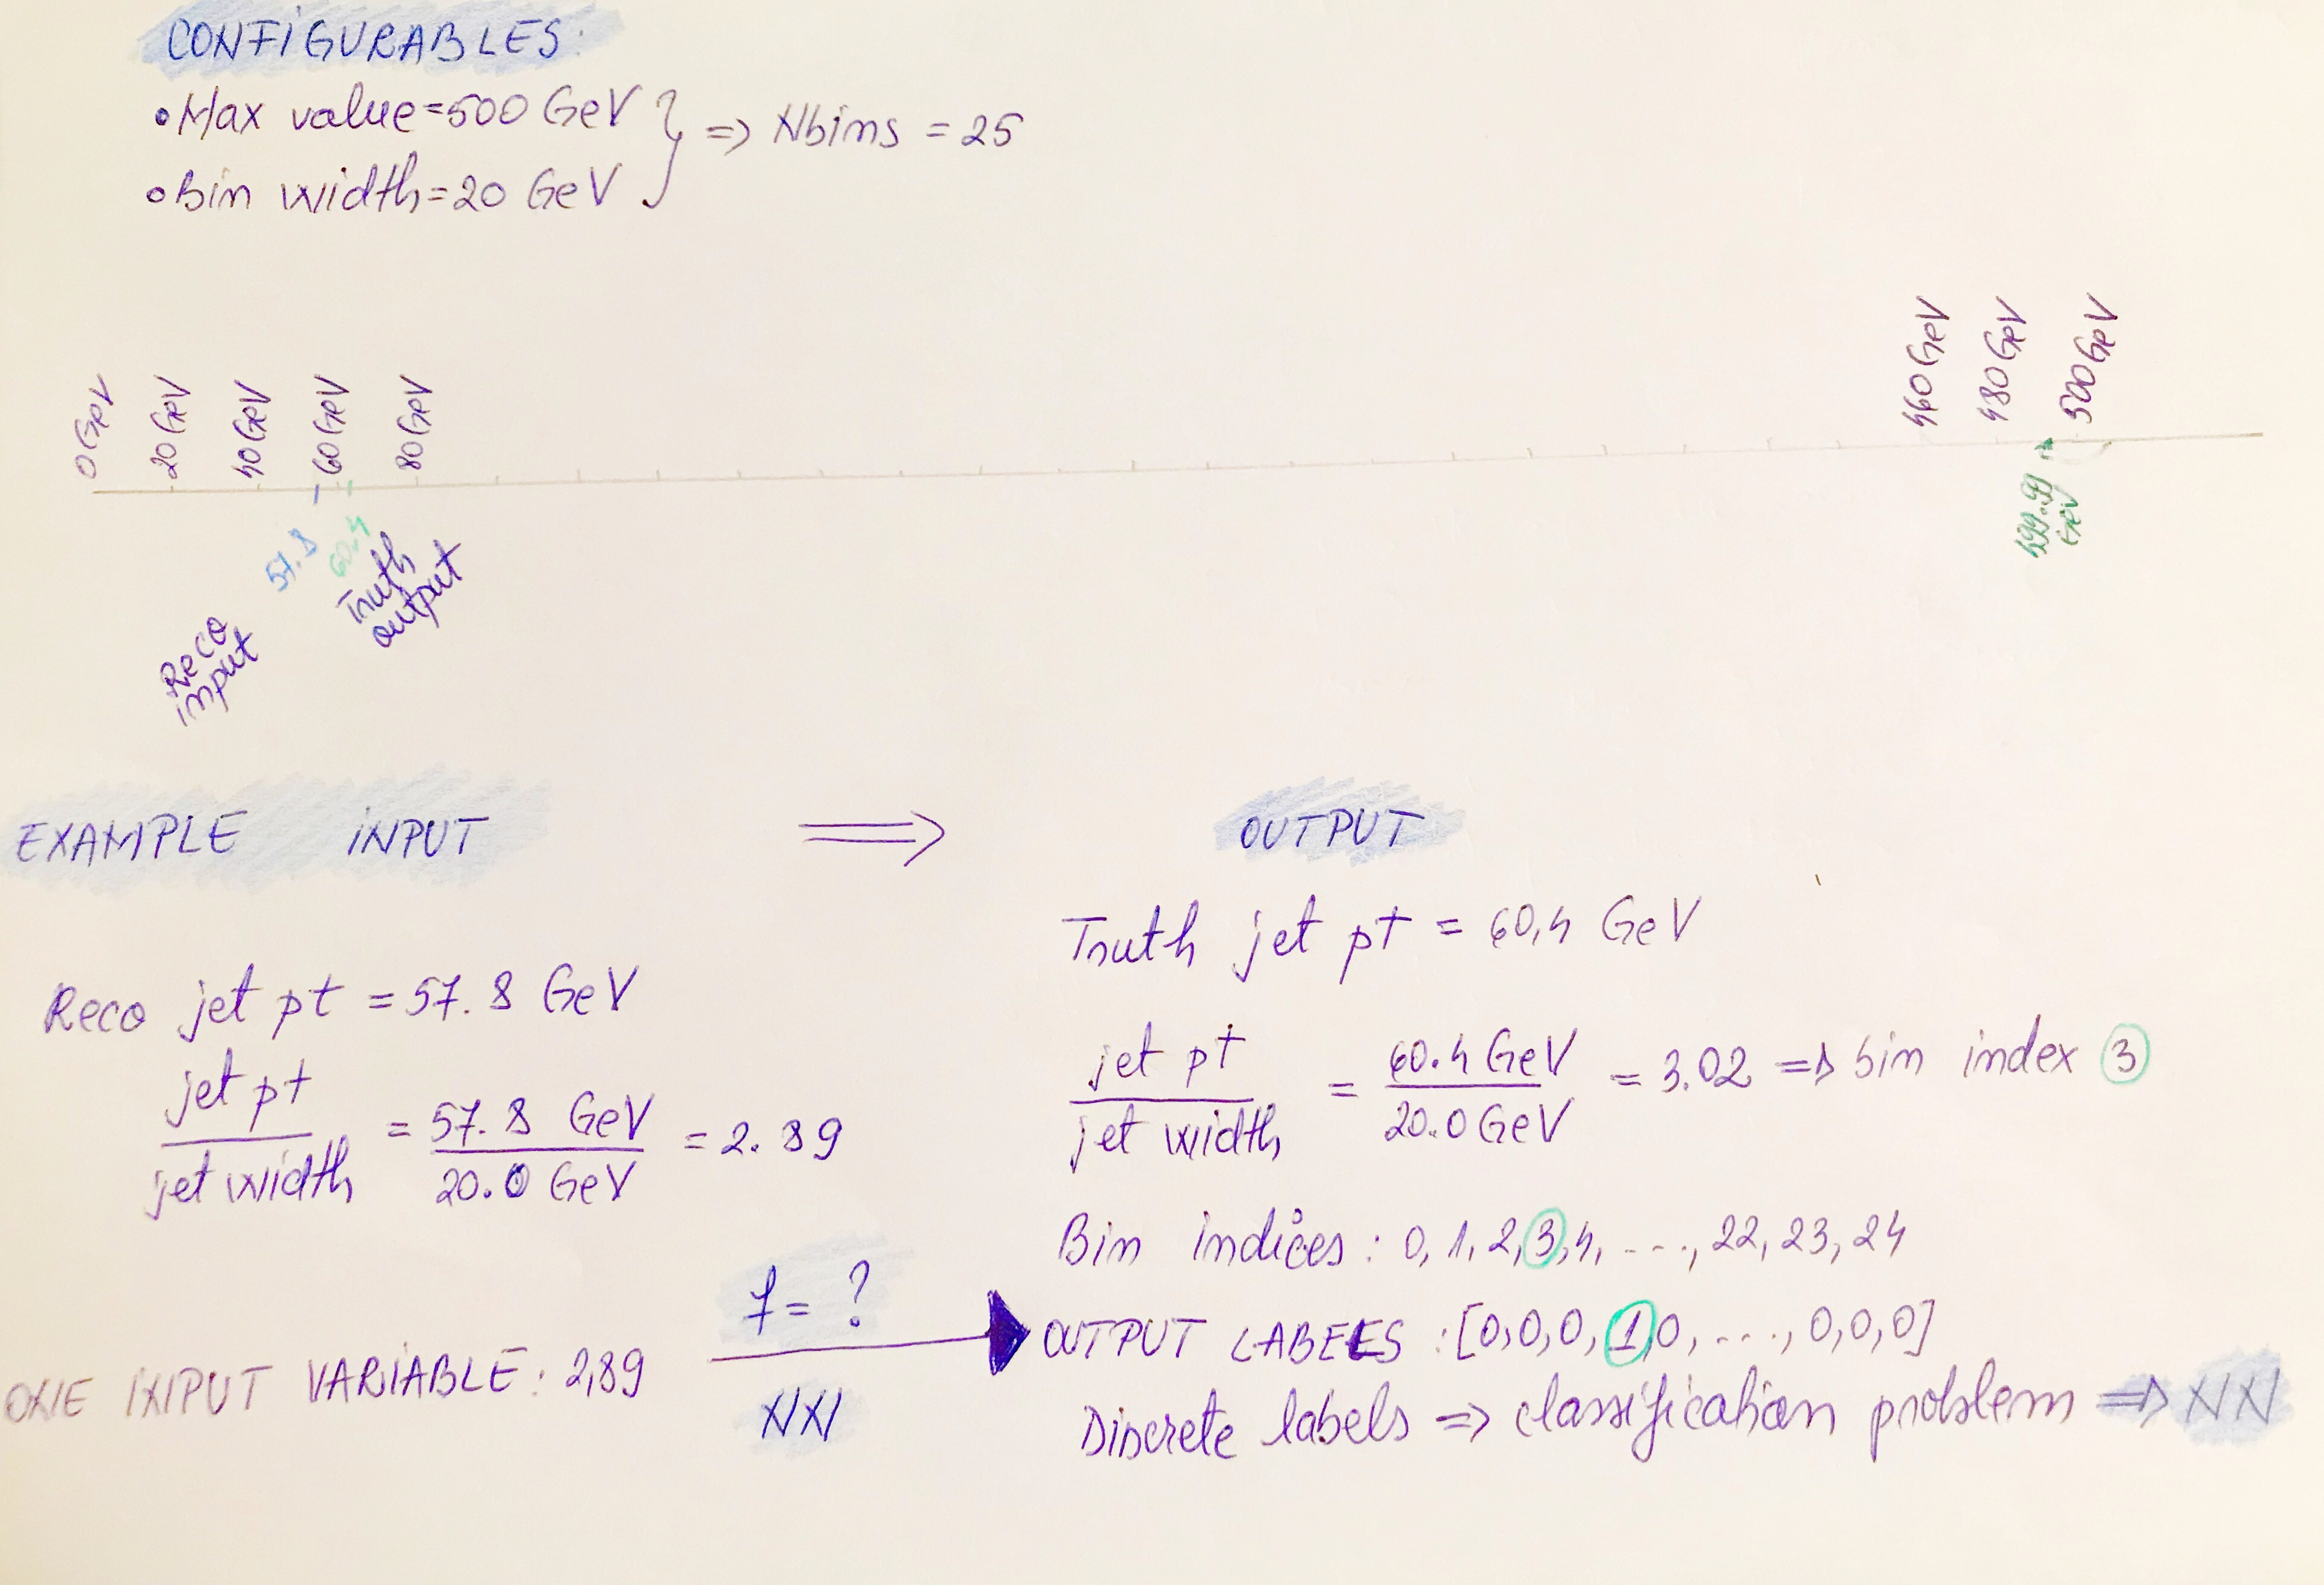
\includegraphics[width=0.49\textwidth]{../presentation/plots/PhysicsProblem.jpg}
  \caption{Diagram of the physics problem.}
  \label{fig:PhysicsProblem}
\end{figure}

The solution is using these NN architectures.

\begin{figure}[h]
  \centering
  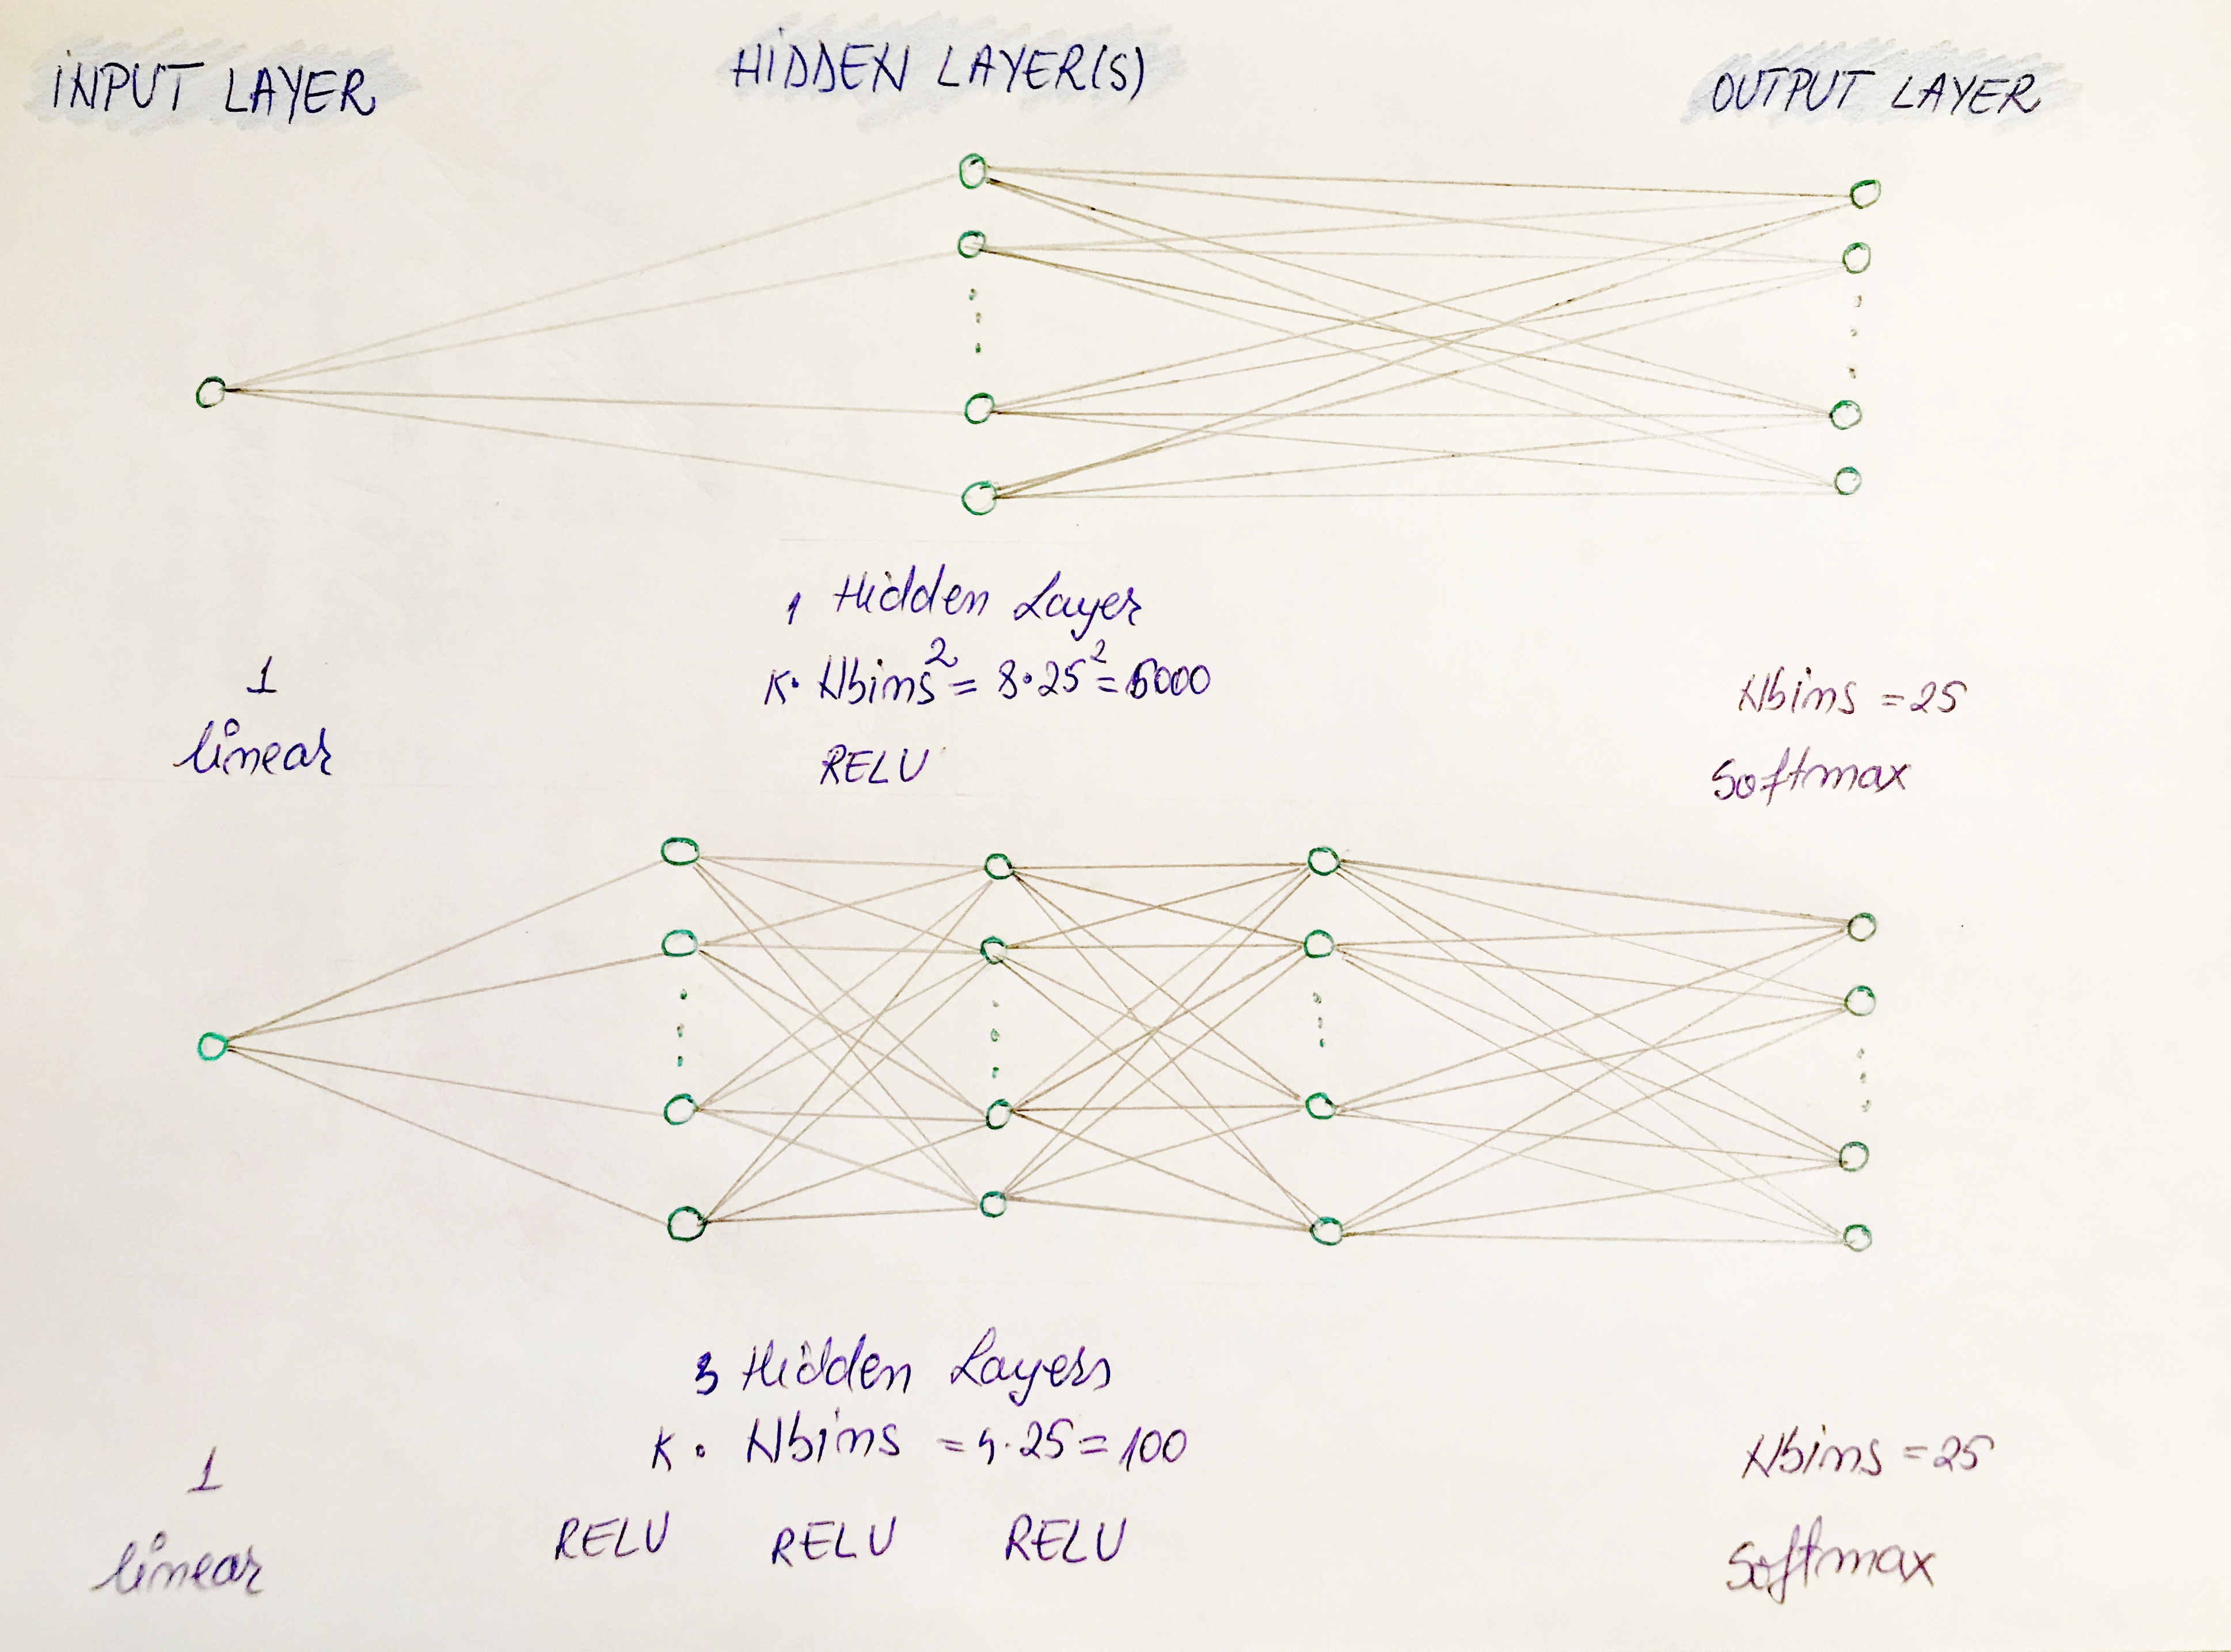
\includegraphics[width=0.49\textwidth]{../presentation/plots/NNArchitecture.jpg}
  \caption{Diagram of the physics problem.}
  \label{fig:NNArchitecture}
\end{figure}

The NN is implemented in TensorFlow, via Keras, in Python. Ran the DNN software for unfolding by DESY Hamburg. Ran on lxplus using the ML software docker image via singularity. Read the ROOT file via the uproot package. Trained  the NNs in Python using Keras and TensorFlow.

\begin{figure}[h]
  \centering
  
\includegraphics[width=0.49\textwidth]{../presentation/plots/TensorFlow_Keras.png}
  
\includegraphics[width=0.49\textwidth]{../presentation/plots/Python.png}
  \caption{Diagram of the physics problem.}
  \label{fig:NNArchitecture}
\end{figure}

 Fine tuned the NN hyper parameters for our ROOT data sample. One NN training is the first step of the iterative unfolding procedure. {Summary of the physics and NN choices. 

One file with 43076 events (and leading jets). Half (21538) in training, half in testing. jet pt: range=0-500 GeV, bin width=20 GeV, number of bins = 500/20 = 25.  Chose the NN training hyper-parameters by changing one at a time while keeping the other constant, and choosing those with largest accuracy and smallest loss values. 

\begin{table}[h!]
  \resizebox{\textwidth}{!}{
    \begin{tabular}{|l|l|l|} % <-- Alignments: 1st column left, 2nd middle and 3rd right, with vertical lines in between
      \hline
      \textbf{Choice} & \textbf{Old NN (toy data example)} & \textbf{New NN (my best choice)}\\
      \hline
      number of nodes per input layer & 1 & 1 \\
      number of nodes per output layer & ${\rm Nbins}=25$ & ${\rm Nbins}=25$ \\
      Number of hidden layers & 1 & 3 \\
      ${\rm k}$ & 8 & 4 \\
      Number of nodes per layer & ${\rm k}\cdot {\rm Nbins}^2=5000$ & ${\rm k}\cdot {\rm Nbins}=100$ \\
      activation function input & linear & linear \\
      activation function hidden & ReLU & ReLU \\
      activation function output & softmax & softmax \\
      batch size & 1000 & 200 \\
      number of epochs & 150 & 150 \\
      \hline
    \end{tabular}
  }
\caption {NN architecture and hyper-parameters comparing for the old NN, suggested in the toy data paper, and the new NN, from the optimisation of this study.}
\end{table}

\section{Conclusions}
\label{sec:Conclusions}

In this report an unfolding study of the unfolding with a machine learning method for the leading jet \pt~in the \ttbaremu~analysis is presented. The question to answer is given the reconstructed leading jet \pt~ from 0 to 500 \GeV, with 20 \GeV bins, in what bin falls the truth (generated) leading jet \pt. Since there are a finite (25) number of possible answers, it is a classification problem, which can be solved by training of and inferring from an artificial neural network. The NN training is done in TensorFlow via Keras in Python. A method and code example using toy data was followed, and adaptated for the ATLAS simulated data. The NN architectureis optimised  and hyper-parameters are fine-tuned to maximize the accuracy values and minimize the loss values in the test sample. The chosen NN performs better than the NN choice suggested in the toy data example. 

\ \\The project lasted six weeks. Given more time, several improvements or further developments are possible. Training one NN is only the first (zeroth) step of a ML-based unfolding method. The performance would improve more NNs are trained. Only one simulation file is used. But using more simulated data in training and testing contains more events and more leading jets, leading to a better training. Only one input variable is used, but several other variables can be added in the ML method, unlike in the migration matrix method. A possible extra variable can be the leading jet $\eta$. A further possible improvement is that instead of a k-fold=2 (using training and test each at 50\% of the events), a larger k-fold to be used (\emph {e.g.} 5). 

\section*{Acknowledgements}
\label{sec:Acknowledgements}

I would like to express my gratitude to DESY for the opportunity to take part in the Summer School program at DESY Zeuthen for the summer of 2019. The particle physics lectures are very enriching. I am grateful to the ATLAS group at DESY for having hosted me for a eight week research project on machine learning unfolding in the \ttbaremu~analysis. I would like to thank my supervisors, prof. Thorsten Kuhl and postdoc Yichen Li, for introducing me to this exciting topic and their great supervision. I am also thankful for their help to the PhD students Matthieu Robin and Martin Habedank I feel also lucky to have had amazing colleagues from many countries at the summer school, with whom I had a lot of fun and will keep in contact in the future.

\begin{thebibliography}{11}

\bibitem{ATLAS} The ATLAS experiment, \url{https://atlas.cern}
\bibitem{RootFile} The \ttbaremu~ROOT file used {\tiny \texttt{\detokenize{/afs/cern.ch/user/l/lciucu/public/data/MLUnfolding/user.yili.18448069._000001.output.sync.root}}}
\bibitem{bendavid} Joshua Bendavid, \textit{Efficient Monte Carlo Integration Using Boosted Decision Trees and Generative Deep Neural Networks}, 2017
\bibitem{AndrewNg} Andrew Ng, \textit{Machine Learning. Coursera online course}, \url{URL https://www.coursera.org/learn/machine learning}
\bibitem{AGlazov} Alexander Glazov, \textit{Machine learning as an instrument for data unfolding}, \textbf{arXiv}: 1712.01814v1, \url{http://inspirehep.net/record/1641082}
\bibitem{AGlazovCode} Alexander Glazov, \textit{Toy data example for machine learning as an instrument  for data unfolding using TensorFlow via Keras in a Python Jupyter Notebook}, \url{https://github.com/aglazov/MLUnfold/blob/master/Unfold.ipynb}
\bibitem{Singularity} The singularity command to run the ML environment, \\ {\tiny \texttt {\detokenize{singularity exec '/cvmfs/unpacked.cern.ch/registry.hub.docker.com/atlasml/ml-base:latest'bash}}}
\bibitem{keras} The keras machine learning library, \url{https://keras.io}
\bibitem{tensorflow} The TensorFlow machine learning library, \url{https:// www.tensforflow.org}
\bibitem{numpy} The Numerical Python library, \url{https://www.numpy.org}
\bibitem{topquark} \textit{Measurement of jet activity produced in top-quark events with an electron, a muon and two b-tagged jets in the final state in pp collision at s=13 TeV with the ATLAS detector}, \textbf{arXiv}: 1610.09978v2, \url{https://arxiv.org/pdf/1610.09978.pdf}
\bibitem{ReportYichenLi} Yichen Li, \textit{ZUnfold framework, an unfolding framework written at Zeuthen}, \url{http://www.desy.de/~liyichen/Unfolding.pdf}
\bibitem{UnfoldingStatSchool}, Stefan Schmitt, Daniel Brizger, \textit{Slides Unfolding in High Energy Physics at the Terascale statistics school 2014}, \url{http://www.desy.de/~sschmitt/talks/UnfoldStatSchool2014.pdf?fbclid=IwAR3CB3CwJOQchKfbZRIg6ktRf6DbI5KTD5cdtBbNHS1lKb-q3yrwagyua5w}.

\end{thebibliography}


\end{document}








\end{thebibliography}

\end{document}

%%%%%%%%%%%%%%%%%%%%%%%%%%%%%%%%%%%%%%%%%%
%%% example code - do not write below
%%%%%%%%%%%%%%%%%%%%%%%%%%%%%%%%%%%%%%%%%%%

\section{Introduction}

\subsection{Part 1...}

\paragraph{}
Here new paragraph starts...........
\paragraph{}
Here new paragraph starts...........
\paragraph{}
Here new paragraph starts........... \\

\newpage
		
Equation:
	
\begin{equation}
% \langle t_f q_f | t_i q_i \rangle = 
\lim_{\substack{\epsilon \rightarrow
0\\N\rightarrow \infty}} \int \dots \int \mbox{d}q_1 \dots \mbox{d}q_{N-1} \frac{\mbox{d}p_1}{2 \pi
\hbar} \dots \frac{\mbox{d}p_N}{2 \pi \hbar}\exp{\left( \frac{i}{\hbar} \sum_{j=1}^N
\left[ p_j (q_j - q_{j-1}) - \epsilon H\left(pj, \frac{q_j +
q_{j-1}}{2}\right)\right]\right)}
\end{equation}
\vspace{2cm}
\begin{align}
 \lim_{\substack{\epsilon \rightarrow 0 \\ N\rightarrow \infty}} \frac{i}{\hbar}
\epsilon \sum_{j=1}^N \left[p_j \left(\frac{q_j-q_{j-1}}{\epsilon}\right) - H\left( p_j,
\frac{q_j+q_{j-1}}{2}\right) \right] &= \frac{i}{\hbar} \int_{t_i}^{t_f} \mbox{d}t \left( p
\dot{q}-H(p,q)\right) \nonumber\\ 
&= \frac{i}{\hbar} \int_{t_i}^{t_f} \mbox{d}t L = \frac{i}{\hbar} S[q]
\end{align}
\vspace{2cm}

Table:

Consider the following mesons $\eta$, $\eta'$ and $K$ and their quark content\footnote{The mesons
are actually a superposition of these quarks.}:
\begin{center}
\begin{tabular}{c|c|c}
 meson & composition & approx. mass\\ \hline
$K^0$ &  $d\bar{s} \, , \,s\bar{d}$ &  $498 \mbox{MeV}$\\
$K^{+}$ & $u\bar{s}$ & $494 \mbox{MeV}$\\
$K^{-}$ & $s \bar{u}$ & $494 \mbox{MeV}$  \\
$\eta$ & $u \bar{u} \, , \, d \bar{d} \, , \, s \bar{s}$ & $548 \mbox{MeV}$ \\
$\eta'$ & $u \bar{u} \, , \, d \bar{d} \, , \, s \bar{s}$ & $958 \mbox{MeV}$ 
\end{tabular}
\end{center}


\newpage
	
Plot:

\begin{figure}[h]
\subfloat{\includegraphics[width=0.495\textwidth]{figure.jpg}}%\label{corr_and_rate-left}}
\subfloat{\includegraphics[width=0.495\textwidth]{figure.jpg}}%\label{corr_and_rate-right}}
\caption{Left: correlation for different $d$ ; Right: acceptance rate and
autocorrelation time for different $d$}
\label{corr_and_rate}
\end{figure}

\newpage
		
\subsection{Part 2...}

\paragraph{}
Here new paragraph starts...............................................................
...........................................................................................
..........................................................................................
...........................................................................................
\paragraph{}
Here new paragraph starts..........................................................................
...........................................................................................
..........................................................................................
...........................................................................................
\paragraph{}
Here new paragraph starts..........................................................................
...........................................................................................
..........................................................................................
........................................................................................... \\

\section{Conclusions}

Some text here..............................................................................

\section*{Acknowledgements}

Some text here..............................................................................

\begin{thebibliography}{11}
\bibitem{nagashima}
Yorikiyo Nagashima, Yoichiro Nambu, \textit{Elementary Particle Physics Volume 1: Quantum Field
Theory and Particles}, (WILEY-VCH, 2010)
\bibitem{FORTRAN}
W. H. Press, S. A. Teukolsky, W. T. Vetterling, B. P. Flannery, \textit{Numerical Recipes in
FORTRAN - The Art of Scientific Computing, 2nd Ed.} (Cambridge University Press, 1992)
\bibitem{buendia}
G. M. Buend\'{i}a, \textit{Comparison between the Langevin and the hybrid simulation techniques for
a free field theory}, J. Phys. A: Math. Gen. \textbf{22}, 5065-5072 (1989).
\bibitem{tapei}
T. Cheung and L. Li, \textit{Gauge theory of elementary particle physics}, (Oxford University
Press, 1984)
\bibitem{degrand}
T. DeGrand and C. DeTar, \textit{Lattice Methods for Quantum Chromodynamics}, (World Scientific,
2006)
\bibitem{topoactions}
W. Bietenholz, U. Gerber, M. Pepe, U.-J. Wiese, \textit{Topological Lattice Actions},
arXiv:1009.2146v4 [hep-lat] (20 Dec 2010)
\bibitem{openbcs}
M. L\"{u}scher, S. Schaefer, \textit{Lattice QCD without topology barriers},
CERN-PH-TH-2011-116, 26pp (May 2011)
\bibitem{Crecipes}
W. H. Press, S. A. Teukolsky, W. T. Vetterling, B. P. Flannery, \textit{Numerical Recipes in
C - The Art of Scientific Computing, 2nd Ed.} (Cambridge University Press, 1992)
\bibitem{andreas}
A. Nube, private communication.
\bibitem{wolff}
U. Wolff, \textit{Critical Slowing Down}, Nuclear Physics B (Proc. Suppl.) \textbf{17}, 93-102
(1990).
\end{thebibliography}
\end{document}
